%%%%%%%%%%%%%%%%%%%%%%%%%%%%%%%%%%%
%%%% INTRODUCCIÓN A LA MEMORIA %%%%
%%%%%%%%%%%%%%%%%%%%%%%%%%%%%%%%%%%

%Buenos días, mi nombre es Miguel González Moreno, soy un antiguo estudiante de la promoción 2014-2019 de ADE+ITI en la Universidad de Deusto. La memoria de mi proyecto de fin de grado la desarrollé en LATEX y a raíz de dicha memoria se ha creado esta plantilla. La plantilla persigue el objetivo de ayudar a cualquier futuro estudiante que se quiera adentrar en este sistema de procesamiento de textos (LATEX). Intentaré explicar cada uno de los campos que aparecen a continuación de modo que todos estén lo más claros posibles y que así, la plantilla, sea de la mayor utilidad posible. Dicho lo cual, comenzamos. 

%Concretamente la memoria y esta plantilla se han realizado en OVERLEAF, un editor de LATEX online pero existen numerosos otros programas que pueden usarse para escribir en este lenguaje. Sin embargo, es posible que algunos de los comandos o funciones cambien de un programa a otro por lo que en caso de cambiar de programa, es probable que algunos comandos no se ejecuten como deberían. En cualquier caso, utilizar otro programa no parece excesivamente complicado pues en caso de que algunos comandos cambien se pueden encontrar fácilmente los equivalentes por Internet. Es cuestión de dedicarle un poco más de tiempo.

%Lo primero de todo, dejar claro que en absoluto soy un experto, es más, ni si quiera soy principiante. Todo lo incluido en esta plantilla se ha aprendido desde cero y lo más probable es que aquello que no está en la plantilla (o que pudiese estar hecho de mejor forma) no lo está puesto que actualmente desconozco como hacerlo, y no porque LATEX no pueda, ya que lo más seguro es que sí se pueda realizar. Así, explicaré todo aquello que sepa dejándoles de profundización en ciertas cuestiones a ustedes. Aquello que desconozca me limitaré a no comentarlo.

%Como se puede observar al compilar, estos textos que aparecen en azul no se escriben en el documento, son comentarios. Los comentarios no son procesados sin embargo sí que se pueden leer en la pantalla de escritura. Intentaré explicar el proceso de creación de la memoria a partir de estos comentarios, siendo todos ellos suprimibles en cuanto el alumno haya comprendido la idea detrás de cada uno de ellos.

%Aún así, si existiese cualquier duda con respecto a la plantilla o a las funciones utilizadas, mi única y principal fuente de conocimiento ha sido Internet, y los maravillosos (y diversos) blogs que se encuentran en la red. Os dejo a continuación aquellos que más me han servido de ayuda (pero la verdad es que hay infinidad). Cualquier función que busquéis, existe. Cualquier problema, lo ha tenido antes otra persona y ha preguntado por ello. Simplemente hay que tener tiempo para encontrar la fuente e ir probando. Esto es prueba y error. 

%Blogs de utilidas: 
%http://minisconlatex.blogspot.com/
%https://tex.stackexchange.com/
%http://metodos.fam.cie.uva.es/~latex/index.html

%Consejo: Por lo general, buscad la ayuda en inglés, hay muchísima más información.

%Finalizada la presentación de la plantilla ¡EMPEZAMOS CON LATEX!

%%%%%%%%%%%%%%%%%%%%%%%%%%%%%%%%
%%%% INTRODUCCIÓN AL LATEX %%%%%
%%%%%%%%%%%%%%%%%%%%%%%%%%%%%%%%

%La escritura en LATEX muy sencilla (una vez se domine lo básico) pero es necesario invertir tiempo para comprenderla, para conocer las funciones y sobre todo para profundizar en ella. Lo básico se aprende rápido. ¡Vamos a ello!

%LATEX trabaja con funciones, todas aquellas palabras que aparecen en verde y van precedidas por el símbolo "\". Cada función suele tener una serie de parámetros opcionales, que se encuentran dentro de "[corchetes]", y una serie de parámetros obligatorios, que se encuentran dentro de "{llaves}". Lógicamente, siempre habrá que introducir un parámetro obligatorio. Los parámetros opcionales se añaden para modificar o precisar elementos de la función en cuestión (dependiendo del uso que le quiera dar el autor).

%En general hay unas funciones básicas que se pueden llamar por defecto, sin embargo para otras es necesario cargar/incluir algunos paquetes especiales. Lo veremos a posteriori (simplemente tenerlo en cuenta).

%%%%%%%%%%%%%%%%%%%%%%%%%
%%%% PRIMERA FUNCIÓN %%%%
%%%%%%%%%%%%%%%%%%%%%%%%%

\documentclass[a4paper,openright,12pt]{book}

%Esta es la primera función del archivo y define el tipo de documento sobre le que se está trabajando. Realmente no tengo un conocimiento exhaustivo sobre los diferentes tipos de documentos en los que se puede trabajar pero encontrar información sobre esta función es muy sencillo.  En este caso, el tipo utilizado es "Book". Se ha utilizado este tipo porque es el más adecuado a documentos largos, con capítulos, secciones y demás. Hay otras clases de documentos como por ejemplo "article", "report" o "memoir". Cada uno con sus características propias. 

%El tipo book permite llamar a otros archivos etcétera. ¿A qué me refiero con llamar a archivos? Como veis en la izquierda estamos trabajando sobre un archivo ".tex" denominado "MAIN.tex". Este archivos es el cuerpo central de nuestra memoria, sin embargo, en él no escribiremos todos los capítulos sino que los capítulos los escribiremos en otros archivos ".tex" (1.Intro.tex, 2.Objetivos.tex y sucesivos) y se llamarán desde "MAIN". Lo veremos más adelante, no os preocupéis. Esto es simplemente para llevar un mayor orden en el documento. Se podría perfectamente escribir toda la memoria en este mismo archivo pero sería algo más caótico y tardaría demasiado en cargar.

%Esta función presntada tiene varios parámetros adicionales: "a4paper", el cual indica que el folio será del tamaño A4, "openright", el cual es utilizado para garantizar que los capítulos nuevos siempre empiecen en una página de la derecha (si en algún momento fuesen a empezar en una página izquierda, LATEX dejará una página en blanco para garantizar esta regla), "10pt" indica el tamaño predeterminado de la fuente a utilizar. 

%Se han indicado así 3 parámetros adicionales. Si no se indican todos los que hay LATEX cogerá los parámetros por defecto en su configuración. Así, que únicamente se hayan indicado 3 no significa que sólo haya 3, probablemente hay muchos más en los que sí se quiere, se puede profundizar buscando información.

%%%%%%%%%%%%%%%%%%%%%%%%%%%%%%%%
%%%% DEFINICIÓN DE PAQUETES %%%%
%%%%%%%%%%%%%%%%%%%%%%%%%%%%%%%%

%LATEX, como se comentaba, no tiene cargadas todas las funciones por defecto (viene lo básico, pero se puede profundizar tanto como se quiera). Así, para ejecutar algunas funciones o símbolos es necesario que se incluyan algunos PAQUETES adicionales. Aquellos en los que se indica PAQUETEB son paquetes prácticamente de inicio, que toda memoria debería como mínimo tener (el resto varía según las necesidades de cada autor).

%Los paquetes se cargan con la función "\usepackage" y aquellos que se han utilizado en la memoria son los siguientes:

\usepackage[utf8]{inputenc}
%PAQUETEB para incluir acentos al escribir en Castellano.
\usepackage[spanish,es-tabla]{babel}
%PAQUETEB para escribir en castellano.
\usepackage{fancyhdr}
%PAQUETEB para definir encabezado y pie de páginas.
\usepackage{ragged2e}
%PAQUETEB utilizado para alinear, justificar o centrar el texto de la memoria.
\usepackage{setspace}
%PAQUETEB para delimitar el interlineado del texto.
%\usepackage{cite}

\usepackage[%
  bibstyle=ieee,
  citestyle=numeric,
  isbn=true,
  doi=false,
  sorting=none,
  url=true,
  defernumbers=true,
  bibencoding=utf8,
  backend=biber
]{biblatex} 

\addbibresource{Bib/MiBiblioteca.bib}


%PAQUETEB para citar y referencia a lo largo del texto.
\usepackage{enumerate} 
%PAQUETEB para formar listas organizadas y darles formato. 
\usepackage[font={color=RBlue},figurename=Fig.]{caption} 
%Paquete para poner subtítulos a las imágenes y concretamente personalizado para que sean de colo azul (elección personal).
\usepackage{graphicx} 
%Paquete para utilizar distintos colores tanto en la escritura, como en tablas, títulos y demás.
\usepackage{subfigure} 
%Paquete para incluir sub-figuras.
\usepackage{hyperref} 
%Paquete para incluir hyperlinks en el PDF.
\usepackage{eurosym} 
%Paquete para incluir el símbolo "€" en el texto.
\usepackage{pdfpages} 
%Paquete para incluir PDFs a lo largo de la memoria, y modificar su formato.
\usepackage{multirow, array} 
%Paquete para dar formato a las tablas.
\usepackage{float} 
%Paquete para forzar que una foto se introduzca exactamente en un sitio determinado y que LATEX no la reposicione.
\usepackage{longtable} 
%Paquete para la gestión y el formateo tablas de mayor dimensión.
\usepackage{xcolor,colortbl} 
%Paquete para crear colores específicos según RGB.
\usepackage{geometry}
%Paquete para definir las dimensiones de los márgenes.

\definecolor{RBlue}{RGB}{23,33,110} 
\definecolor{Rojo}{RGB}{255,0,0}
\definecolor{Cyan}{RGB}{214,234,240}
\definecolor{Naranja}{RGB}{255,222,199}
\definecolor{GrisTabla}{RGB}{245,245,245}
%Ejemplo de funciones para definir colores a utilizar el documento, según sus dígitos RGB.

%Paquetes para algoritmos matemáticos
\usepackage{amsmath}
\usepackage{algorithm}% http://ctan.org/pkg/Algoritmos
\usepackage[noend]{algpseudocode}
\makeatletter
% Reinsert missing \algbackskip
\def\algbackskip{\hskip-\ALG@thistlm}
\makeatother

\usepackage{multicol}
\usepackage{eurosym}
\usepackage{slashbox}
\usepackage{adjustbox}

\usepackage{tikz}
\usepackage{collcell}
\usepackage{etoolbox}

%%%%%%%%%%%%%%%%%%%%%%%%%%%%%%%%%%%%%%%%%%%%%%%%%%%%%%%%%%%
%%%% PROPIEDADES DEL DOCUMENTO (Funciones específicas) %%%%
%%%%%%%%%%%%%%%%%%%%%%%%%%%%%%%%%%%%%%%%%%%%%%%%%%%%%%%%%%%

\setcounter{secnumdepth}{5} 
%Esta función permite que en el índice se indique hasta el sub-nivel número tres. Es decir que aparezcan hasta los apartados 1.1.1. Si se indicase {4}, se podrían observar hasta los sub-apartados 1.1.1.1. 

\setlength{\headsep}{0.5in} 
%La función "\setlength" permite cambiar (sobrescribir valores predeterminados) todas las distancias del documento. En función de que {parámetro} se indique se cambiará una distancia u otra. En este caso se está cambiando la distancia entre el encabezado y el texto para que esta sea durante todo el documento media pulgada. Se puede indicar la distancia que se quiera (cuestiones estéticas) y también se puede indicar la distancia en el sistema métrico (mm, cm).

\onehalfspace 
%Esta función determina que el interlineado a lo largo del documento sea de 1.5. Existen otras funciones para cambiar el interlineado como "\Doublespacing" para interlineado doble, "\singlespace" para interlineado sencillo o "\setspace{}" para indicar aquel que sea preferido de forma específica.

\setlength{\parindent}{0cm}
%Nuevamente se utiliza esta función para cambiar distancias del documento. Concretamente, en este caso se utiliza para cambiar la distancia de las sangrías al comenzar nuevo párrafo. Al marcar el valor en 0, se eliminan las sangrías del documento. Siempre se puede en momentos posteriores forzar la inclusión de alguna sangría o reescribir de nuevo el valor para indicar que a partir de ahí, comiencen las sangrías de nuevo.

\includeonly{
                Capitulos/0.Resumen, 
                Capitulos/0.Abstract, 
                Capitulos/1.Intro,
                Capitulos/2.AntecedentesJustificacion, 
                Capitulos/3.Objetivos_y_Alcance, 
                Capitulos/4.ConsideracionesEticas, 
                Capitulos/5.Metodologia, 
                Capitulos/6.Planificacion,
                Capitulos/7.IntroduccionFedLearn,
                Capitulos/8.0.Desarrollo,
                Capitulos/9.Presupuesto,
                Capitulos/10.Conclusiones,
                Capitulos/Funciones,
                Anexos/1.AnexoProteccionDatos,
                Anexos/2.AnexoPlanificacion
}
%Esta función es de gran importancia. Como se puede observar a la izquierda, hay una carpeta que se ha creado con diferentes capítulos. Estos capítulos son los diferentes apartados de la memoria en los que se va a ir escribiendo. Por ejemplo, el capítulo de la introducción, el capítulo de objetivos, el capítulo de la memoria técnica, o el capítulo del plan de trabajo. Bien, de cara a poder incluirlos a posteriori en esto documento principal (MAIN.tex) es necesario indicarle a LATEX que los cargue y eso se realiza con esta función. Así, habrá que incluir tantos parámetros como capítulos se deseen cargar. Los parámetros son simplemente la dirección de la carpeta en la que se encuentran, y su nombre.

\geometry{top=3cm, bottom=3cm, left=3.5cm, right=2.5cm}
%Esta función determina los márgenes que se han de utilizar a lo largo de todo el documento. Así, el margen superior será de 3 centímetros, igual que el inferior y los márgenes exterior e interior serán de 3.5 y 2.5 centímetros respectivamente.

\pagestyle{empty}
%Esta función es bastante útil ante diversos problemas que puedan surgir a lo largo del documento con las páginas en blanco. Esta función determina que el estilo (encabezados y pies de página) de la página estrictamente posterior sea totalmente blanco (vacío - empty).

%%%%%%%%%%%%%%%%%%%%%%%%%%%%%%%%%%%%%%%%%%%%%%%%%%%%%%%%%%%%%%%%
%%%% COMIENZA EL DOCUMENTO (con la función \begin{document} %%%%
%%%%%%%%%%%%%%%%%%%%%%%%%%%%%%%%%%%%%%%%%%%%%%%%%%%%%%%%%%%%%%%%

\begin{document}

%%%%%%%%%%%%%%%%%%%%
%%%% PAGINACIÓN %%%%
%%%%%%%%%%%%%%%%%%%%

\pagestyle{fancy}
%Esta función es utilizada para crear un nuevo estilo de formato, es el formato "fancy". En él vamos a determinar a continuación cómo se quieren posicionar pies de página, encabezados y demás.

\lhead{}
%Esta función sirve para que no se escriba nada (parámetro obligatorio vacío) en el encabezado en la posición izquierda. 

\chead{}
%Esta función sirve para que no se escriba nada (parámetro obligatorio vacío) en el encabezado en la posición central. 

\rhead{}
%Esta función sirve para que no se escriba nada (parámetro obligatorio vacío) en el encabezado en la posición derecha. 

\cfoot{}
%Esta función sirve para que no se escriba nada (parámetro obligatorio vacío) en el pie de página en la posición central. 

\fancyhead[OR]{}
%Esta función sirve para que no se escriba nada (parámetro obligatorio vacío) en el las páginas impares, en el encabezado en la posición derecha.

\fancyhead[OL]{}
%Esta función sirve para que no se escriba nada (parámetro obligatorio vacío) en el las páginas impares, en el encabezado en la posición izquierda.

\fancyhead[ER]{}
%Esta función sirve para que no se escriba nada (parámetro obligatorio vacío) en el las páginas pares, en el encabezado en la posición derecha.

\fancyhead[EL]{}
%Esta función sirve para que no se escriba nada (parámetro obligatorio vacío) en el las páginas pares, en el encabezado en la posición izquierda.

\fancyfoot[LE,RO]{\thepage} 
%Esta función sirve para indicar que el número de la página correspondiente se escriba a la izquierda en las páginas pares y a la derecha en las páginas impares.

\renewcommand{\headrulewidth}{0pt} 
%Esta función sirve para renovar todo tipo de comandos o distancias en el documento. Concretamente, en este caso se indica que no exista (grosor 0pt) una linea debajo del encabezado que lo separe del texto.

\includepdf[]{PDF/Portada_TFG_IngenieriaInformatica}
%Esta función incluye el PDF de la portada correspondiente al TFG. Dicho documento PDF ha de estar cargado en el menú de la izquierda como se encuentra esta portada auxiliar. Es importante incluir en el parámetro obligatorio la dirección a dicho PDF con su normbre correspondiente.

\newpage
\thispagestyle{empty}


\frontmatter
%Esta función sirve para que, en las primeras páginas de la memoria (hasta que se indique lo contrario con otra función), la paginación sea en números romanos como lo indican los criterios de formato en índice, resumen y demás apartados.

%como se puede ver, todo lo expuesto arriba (en términos de paginación) es un poco redundante y bastante lioso, aún así, funciona. Ahora, no tengo ninguna duda de que se puede optimizar, eliminar funciones o sustituir por otras para que sea más "user-friendly". Estaré encantado de escuchar como hacerlo, pero de momento desconozco como mejorar el código sin que genere errores. Dicho esto, como se comentaba al principio, es cuestión de dedicarle  tiempo y comprender más a fondo las funciones. 

\setcounter{page}{3}
%Esta función permite comenzar el contador de las páginas para la numeración en el número 3, es importante puesto que los primeros números van dedicados a portada y contraportada y no se numeran. Así, la primera página numerada será la 3. 

%\chapter*{Resumen}

\thispagestyle{fancy}

a
\\
\textbf{Descriptores}\\
% Lorem, ipsum, dolor, sit, amet
a

\newpage
%Función para incluir un salto a una nueva página.
\thispagestyle{empty}
%Función para que dicha página no tenga ningún formato (ni número, ni encabezado).

%Así con estas dos funciones de forma consecutiva se crea una página en blanco.
%\chapter*{Abstract}
%Nuevo capítulo para incluir el resumen (si se quiere también en inglés).

\thispagestyle{fancy}
Lorem ipsum dolor sit amet, consectetur adipiscing elit. Aenean semper non orci at fringilla. Etiam fermentum in diam vestibulum pellentesque. Nam volutpat, velit ut euismod mollis, ipsum erat facilisis justo, et tempor est lectus nec massa. Pellentesque habitant morbi tristique senectus et netus et malesuada fames ac turpis egestas. Sed accumsan viverra neque eu blandit. Suspendisse in fermentum felis, id iaculis mi. Quisque maximus quam lacus, non lobortis libero tincidunt at. Pellentesque habitant morbi tristique senectus et netus et malesuada fames ac turpis egestas. Maecenas lectus nibh, sagittis ut felis non, fermentum ullamcorper leo. In hac habitasse platea dictumst. Orci varius natoque penatibus et magnis dis parturient montes, nascetur ridiculus mus. Fusce est dui, dapibus ultricies ipsum quis, ultrices maximus dolor. Proin finibus, lorem vulputate maximus convallis, quam tellus posuere magna, sed maximus nunc eros quis ipsum. Cras dignissim cursus lectus ac auctor. Donec suscipit vestibulum neque, sed lobortis est rhoncus non.\\

Praesent ut neque eros. Praesent vitae augue at diam tincidunt sagittis. In cursus lorem nec neque condimentum dictum. Morbi vel tristique orci. Cras luctus tempus elit tincidunt hendrerit. Proin bibendum arcu et sapien finibus vulputate sed eget leo. Duis at bibendum massa, sit amet ornare lorem. Donec dictum finibus fringilla. Duis accumsan lectus dolor, eu maximus ligula semper vel. Proin a sem tincidunt, mollis magna eget, consequat tortor. In sodales justo et varius scelerisque. Aliquam sit amet lacus mollis, tincidunt erat vitae, lacinia sem. Maecenas vel erat sagittis, semper ex in, commodo libero.\\

Integer malesuada quis elit eu eleifend. Suspendisse non vestibulum est, a fermentum urna. Donec ligula tortor, ultrices varius nisi eget, dictum malesuada augue. Fusce lacus orci, eleifend quis luctus dictum, ultricies id turpis. Vestibulum et auctor orci. Pellentesque habitant morbi tristique senectus et netus et malesuada fames ac turpis egestas. Integer facilisis neque quis dui dapibus dictum.\\

\textbf{Descriptors}\\
Lorem, ipsum, dolor, sit, amet


\newpage
\thispagestyle{empty}

\fancypagestyle{plain}
{
}
%Se define mediante esta función el formato plain, que no tiene nada, ni encabezados ni pies de página. Realmente esta función podría ir a comienzo del documento o en cualquier lugar, es decir, se puede mover.

\tableofcontents
%Esta función permite introducir el índice de capítulos (hasta el subíndice que se haya indicado previamente).

\newpage
\thispagestyle{empty}

\cleardoublepage
%Esta función permite que aunque acabe en página impar, el siguiente apartado, comience en página impar. Con este comando te aseguras que se hace bien y que además se mantiene la numeración correspondiente en números romanos. Es decir, la página que se quedaría en blanco no está en blanco sino que mantiene la numeración. En caso de no querer numeración hay que utilizar los comando ("\newpage" y "\thispagestyle{empty}).

\newpage
\thispagestyle{empty}

\listoffigures
% Es la función que introduce el índice de figuras. Funciona exactamente igual que el de capítulos.
\newpage
\thispagestyle{empty}

\cleardoublepage

\listoftables
%Por ultimo, se introduce el índice de tablas en caso de que las hubiera en vuestro documento. 

\newpage
\thispagestyle{empty}
%Página en blanco

\mainmatter
%Esta función se utiliza para indicar que a partir de ahora la numeración pasa a ser con números estándar y no con romanos como se había venido utilizando hasta ahora.

\pagestyle{fancy}
%A continuación se vuelve a redefinir el estilo “fancy” para que se adecúe al que ha de utilizarse a lo largo de toda la memoria. El estilo es el siguiente:

\lhead{}
%Encabezado a la izquierda vacío. En realidad debe de ir el nombre del capítulo en el que se está escribiendo pero ello se gestionará dentro de cada capítulo (pues el nombre cambia). Aquí se define el formato general.

\chead{}
%Encabezado en el centro vacío.

\fancyhead[OR]{PROYECTO FIN DE GRADO}
%En el encabezado a la derecha en las páginas pares se escribe: "PROYECTO FIN DE GRADO".

\fancyhead[OL]{} 
%Encabezado a la izquierda en las páginas pares vacío. Probablemente esta función sea redundante con la función \lhead y sería omitible.

\fancyhead[ER]{}
%Encabezado en las páginas impares a la derecha vacío.

\cfoot{} 
% Pie de página en el centro vacío.

\fancyfoot[LE,RO]{\thepage} 
%En el pie de página se va a escribir el número de la página correspondiente. Se escribirá en la derecha en las páginas pares y en la izquierda en las páginas impares.

\renewcommand{\headrulewidth}{0pt} 



\chapter{Introducción}
\thispagestyle{fancy}
\fancyhead[LE]{\thechapter.Introducción}


\fancyhead[LE]{}
\newpage
\thispagestyle{empty}
\cleardoublepage

\chapter{Antecedentes y justificación}
\thispagestyle{fancy}
\fancyhead[LE]{\thechapter.Antecedentes y justificación}

\section{Antecedentes}
Este proyecto parte del proyecto de R. Sánchez y col.\autocite{sanchez-corcueraPersuasionbasedRecommenderSystem2020}, donde se desarrolló un sistema de recomendación de estrategias de persuasión basado en aprendizaje activo. Para comprender los antecedentes que han incurrido en el desarrollo de este proyecto hay que conocer y comprender qué son los sistemas de recomendación y los problemas de privacidad que van ligados a estos. 
\subsection{Sistemas de recomendación}
Los sistemas de recomendación, en inglés RM (Recommender System), fueron mencionados por primera vez en los años 90 y han ido evolucionando hasta estar implantados en gran parte de las empresas actuales. Estos, son sistemas de filtrado de información, que, partiendo de una gran cantidad de datos, tanto de usuarios como de los elementos a recomendar, pueden predecir cuál será el elemento más apropiado para cada usuario. Estos sistemas están estrechamente relacionados con el marketing, ya que el objetivo general de recomendar algún elemento que sea del agrado e interés de un usuario suele ir ligado a fines económicos.
\\ \\
Hoy en día se usan en multitud de campos, desde las redes sociales hasta las distribuidoras de contenido como Netflix, pasando por compañías de comercio electrónico como Amazon. 
\\ \\
A la hora de realizar la recomendación, se realizan filtrados de diferente tipo, estos filtros son la forma en la que el sistema busca correlacionar los usuarios con los elementos que estos consumen, compran o ven. Entre los métodos más comunes para relacionar esta información y obtener resultados eficientes se encuentran:
\begin{itemize}
    \item \textbf{Filtros demográficos}, que recomiendan en función del sexo, edad, país, oficio,… 
    \item \textbf{Filtros basados en contenidos}, como YouTube, que recomiendan contenidos similares a los valorados por los usuarios. 
    \item \textbf{Filtrado colaborativo}, que consiste en recomendar al usuario elementos valorados positivamente por usuarios similares a él. 
\end{itemize}

Sin embargo, existen sistemas híbridos que combinan varias de las estrategias de filtrado anteriores. Un ejemplo de ello es el anteriormente mencionado Amazon, que tiene uno de los algoritmos de recomendación más potentes y eficientes actualmente. 
\\ \\
Esto se debe a dos cosas, en primer lugar, cuenta con una gran cantidad de información de los usuarios, tanto su edad, género, país, dirección, rutinas (si tienen Alexa), … como los artículos que miran, compran, añaden a la lista, etc. Con todo esto, el algoritmo es capaz de ofrecer recomendaciones muy precisas a los usuarios, lo que le da una gran calidad de servicio a la empresa.
\\ \\
De hecho, en Amazon, si se quiere revisar las recomendaciones existe un apartado propio para ellas al que se puede acceder fácilmente (Fig\ref{fig:AmazonRecomendaciones}).
\begin{figure}[thbp]
    \centering
    \fbox{\includegraphics[width=0.45\textwidth]{Figuras/Amazon_acceder_mis_recomendaciones.png}}
    \fbox{\includegraphics[width=0.45\textwidth]{Figuras/Amazon_recomendaciones.png}}
    \caption{Recomendaciones de Amazon (Fuente: Amazon\autocite{AmazonEsCompra})} 
    \label{fig:AmazonRecomendaciones}
\end{figure}

\subsection{Privacidad digital}
Queda claro que un RS depende plenamente de la información de la que dispone, de forma que, de cuanta más información de los usuarios disponga, más precisión tendrá en sus predicciones. Para obtener esta información muchos anunciantes se han valido de diversas herramientas y utilidades, pero si se ha de destacar alguna, es la utilización de las cookies de terceros. Estas, son definidas por Google\autocite{ComoBorrarHabilitar} cómo:
\\
\begin{minipage}[t]{0.2\linewidth}
\end{minipage}
\hfill
\begin{minipage}[t]{0.9\linewidth}
  \textit{"... son archivos que crean los sitios web que visitas para guardar información de la navegación y facilitar tu experiencia en línea. Gracias a las cookies, los sitios pueden mantener abierta tu sesión, recordar tus preferencias del sitio y proporcionarte contenido relevante en función del lugar donde te encuentres. Hay dos tipos de cookies:
  \begin{itemize}
      \item Las cookies de origen, que las crea el sitio que visitas. El sitio se muestra en la barra de direcciones.
      \item Las cookies de terceros, que las crean otros sitios. Parte del contenido que ves en la página web que visitas, como anuncios o imágenes, pertenece a estos sitios."
  \end{itemize}}
\end{minipage}
\\ \\
A simple vista, estas cookies parecen inofensivas, pero el problema radica en su utilización. Aunque suelen ser usadas con fines analíticos por compañías de marketing online, estas registran el comportamiento de un usuario en la red y crean perfiles de usuarios para ofrecer publicidad personalizada para cada tipo de perfil. Del comportamiento de un usuario en internet se pueden saber sus movimientos, hábitos, páginas que visita, edad, sexo, etc. lo que hace que estos sistemas en ocasiones sean intrusivos y vulneren la privacidad de los navegantes. 
\\ \\
En España y en la Unión Europea existe una legislación sobre la privacidad y la protección de datos en la que se restringen y limitan los datos que estas empresas pueden registrar de la navegación online, el Reglamento General De Protección de Datos (RGPD). En el documento adjunto Anexo \ref{appendix:ProteccionDatos}, sección \ref{appendix:ProteccionDatos_Legislacion} se puede consultar un breve resumen de la legislación en vigor. En lo referente a las cookies, este reglamento presenta varios elementos importantes: 
\begin{itemize}
    \item En primer lugar, debe haber un consentimiento explícito del usuario en el consentimiento de la política de cookies. 
    \item En segundo lugar, la aceptación de las cookies de terceros no ha de ser un impedimento para el uso del servicio.
    \item En último lugar, todas las cookies y rastreadores que operen en la web del propietario deberán ser mostradas al usuario en un lenguaje sencillo.
\end{itemize} 
Aun así, esta legislación no impide que se realice un perfilado del usuario, que se haga un seguimiento de este por la red o que se analice el tiempo que pasa en la página. Con la maduración de la tecnología cada vez más gente se preocupa por el uso que les dan estas empresas a los datos y son más críticos con estas prácticas. Esto ha llegado incluso a la política, donde España está desarrollando una carta pionera de derechos digitales, en la cual, entre otras cosas, recoge el derecho de los usuarios a no ser perfilados (Anexo \ref{appendix:ProteccionDatos}, sección \ref{appendix:ProteccionDatos_Derechos}).
\\ \\
Hoy en día existen muchos navegadores y complementos que permiten bloquear este tipo de rastreadores, lo que ha llevado al sector y a Google a tener que explorar nuevas vías para obtener esta información. La solución propuesta por Google ha sido su nuevo sistema Federated Learning of Cohorts (FLoCs)\autocite{BuildingPrivacyfirstFuture2021}, aprendizaje federado de cortes, con el que se compromete a dejar las cookies de terceros.
\\ \\
Lo que a priori puede significar una buena noticia puede no serlo en realidad. Este sistema permite a Google y a su navegador agrupar y perfilar usuarios en base a sus intereses y perfiles geográficos gracias al historial de navegación y a los datos recogidos durante la navegación. Aunque este sistema no permita que los usuarios puedan ser distinguidos dentro de un grupo, este perfilado supone una persecución y rastreo más grave que el acaecido por las cookies de terceros. En primer lugar, sitúa a Google como principal proveedor de marketing digital, lo que afectaría tanto a la labor de las empresas de marketing digital como al precio que tendrían que pagar estas por la información y los datos.
\\ \\
Ante esta imposición de Google, varias empresas se han pronunciado y han expresado su total desacuerdo con la política, navegadores como DuckDuckGo o Brave la han calificado de anticompetitiva, invasiva y abusiva. Esto se debe a que el navegador de Google, Google Chrome, acapara el 64.19\%\footnote{Fuente: https://gs.statcounter.com/, 27/04/2021} de la red y podría obligar a utilizar su sistema a muchos anunciantes y sitios web.
\\ \\  
\section{Justificación}
Este proyecto es una respuesta al estado de la industria del marketing digital, donde se exprimen al máximo las leyes y normas sobre protección de datos y privacidad digital, y a la actitud de las grandes empresas por perfilar a los usuarios y recoger tanta información de estos como les sea posible.
\\\\
Se quiere demostrar que se puede utilizar el FL preservando la privacidad de los usuarios en un RS, permitiéndoles tener el control total sobre su información desde su propio dispositivo. 
\\ \\
Además, para ello se utilizarán dispositivos como las Raspberries Pi, las cuales servirán para demostrar que no se necesitan dispositivos especialmente potentes para participar en una red de FL, evidenciando que es posible implementar un RS respetuoso con el usuario, acorde al RGPD y salvaguardando los derechos digitales.

\fancyhead[LE]{}
\newpage
\thispagestyle{empty}
\cleardoublepage

\chapter{Objetivos y Alcance}
\thispagestyle{fancy}
\fancyhead[LE]{\thechapter.Objetivos y Alcance} 
\section{Objetivos}
Los objetivos de este proyecto pueden clasificarse en varios grupos. Por un lado están los objetivos generales, objetivos que a simple vista no tienen hitos específicos independientemente del estado en que encuentren y si se han cumplido o no.
\\ \\
Por otro lado se encuentran los objetivos específicos. Estos, al contrario que los generales, son fácilmente identificables, ya que permiten saber si la tarea se ha completado, y en caso contrario, saber en qué estado se encuentra dicha tarea. Dentro de este grupo se encuentran los objetivos específicos de desarrollo, apartado donde se agrupan los objetivos que permiten saber en qué estado de desarrollo se encuentra el proyecto y qué funcionalidades incorpora. Pero además, también se encuentran los objetivos de estudio, donde se incluyen los objetivos que tienen que ver con el estudio de los diferentes experimentos que se realizarán. 

\subsection{Generales}
El objetivo general de este proyecto es el de desarrollar un sistema de recomendaciones online basado en federated learning. Este sistema se desarrollará sobre otro sistema de recomendaciones ya existente basado en Machine Learning, y deberá adaptarlo para su correcto funcionamiento con información descentralizada.
\\ \\
Para respetar la privacidad y derechos de los usuarios, el proyecto deberá incluir la privacidad como patrón de diseño, cumpliendo tanto con las normativas vigentes en Europa y España como con las posibles nuevas medidas que entren en vigor en un futuro. 
\\ \\
Por último, el sistema deberá asegurar que la información se quede en el dispositivo y no se comparta ninguna información que no sea la del propio modelo desarrollado por el participante de la red.

\subsection{Específicos}
Los objetivos específicos son fácilmente reconocibles y concretos, lo que permite saber con exactitud cuándo se han cumplido los objetivos y cuándo no.

\subsubsection{De desarrollo}
Los objetivos de desarrollo tienen que ver con el correcto desarrollo del sistema de recomendación basado en federated learning. 
\\ \\
\textbf{Parametrización y configuración: }
Se tendrán que configurar las plataformas de desarrollo para poder ejecutar el sistema de recomendación centralizado con mayor rapidez y agilizar el desarrollo del proyecto. También se tendrán que configurar las Raspberries y la Jetson Nano, aprovisionarlas del software necesario para ejecutar en ellas el sistema de recomendación y ejecutarlo sin problemas.
\\ \\
\textbf{Desarrollo: }
Se desarrollarán todas las características de los sistemas de recomendación derivadas de la fase de investigación.

\subsubsection{De investigación}
Los objetivos de investigación, al contrario que los de desarrollo, tienen que ver con la búsqueda de soluciones a las incógnitas del proyecto. Es decir, suplir las limitaciones derivadas del federated learning además de la formación del propio alumno en esta tecnología.
\\ \\
\textbf{Formación: }
El alumno deberá formarse en conocimientos sobre Inteligencia Artificial para poder comprender los conceptos. También tendrá que familiarizarse con el código del sistema de recomendación para poder realizar las modificaciones pertinentes en él. Además, el alumno deberá leer artículos científicos sobre federated learning para comenzar a investigar las soluciones a los problemas derivados del proyecto.
\\ \\
\textbf{Sistema de recomendación: }
Se deberá investigar la forma de combinar modelos de IA de cada Raspberry. Además, se investigarán y realizarán las modificaciones pertinentes en el sistema de recomendación para cumplir los siguientes puntos:
\begin{itemize}
    \item Que sea capaz de obtener las recomendaciones para un único usuario en concreto. 
    \item Que sea capaz de guardar y cargar los modelos entrenados de LightFM.
    \item Que el modelo de LightFM sea capaz de admitir aprendizaje incremental.
\end{itemize}

\subsubsection{De estudio}
Los objetivos de estudio tienen que ver con el análisis de los resultados del sistema de recomendación basado en federated learning.
\\ \\
\textbf{Análisis: }
El estudio del sistema tendrá que analizar la diferencia de rendimiento entre el sistema de recomendación con información centralizada y distribuida. También tendrá que analizar cómo afectan los distintos modelos y su combinación al rendimiento del sistema de recomendación.
\\ \\
\textbf{Privacidad: }
Hay que valorar y analizar la privacidad y seguridad de los datos personales de los usuarios tanto en el modelo central, como en el distribuido. Se deberán evitar los problemas de seguridad y privacidad implícitos de la implementación de un sistema de recomendación basado en federated learning

\section{Alcance}
El alcance se centra en concretar qué objetivos entran en el desarrollo del proyecto y cuáles no. Para ello se ha dividido este apartado en dos grupos, los objetivos y tareas que entran en el alcance del proyecto y los que no. La segregación en estos grupos nos permite concretar con más precisión los límites del proyecto, evitando que se amplíe más allá de sus límites. 

\subsection{Dentro del alcance}
Entran dentro del alcance los objetivos y tareas derivadas del desarrollo de un sistema de recomendación basado en federated learning, tanto las tareas de parametrización y configuración del hardware como el desarrollo de software. Esto incluye todos los objetivos específicos de desarrollo mencionados en el apartado anterior.
\\ \\
Del mismo modo quedan dentro del alcance los objetivos de investigación del apartado anterior, ya que son indispensables para el correcto desarrollo del sistema de recomendación
\\ \\
También se incluye el estudio y análisis de los resultados del sistema de recomendación, así como su precisión y sus inconvenientes, es decir, todo lo comentado en los objetivos específicos de estudio.
\\ \\
Para finalizar se incluirá un estudio de la estabilidad legal del sistema en el tiempo. Esto incluye la corroboración del cumplimiento de las actuales medidas de protección de datos y el estudio de las posibles futuras medidas, legislaciones y derechos que limiten el uso de información en Europa.
\\ \\
Se recogera el desarrollo de todo el proyecto en la memoria técnica que será entregada como proyecto fin de grado.

\subsection{Fuera del alcance}
Fuera del alcance queda cualquier estudio de mercado sobre si la solución sería viable económicamente además de cualquier estudio de alternativas a federated learning. 
\\ \\
No se incluirá ni se recogerá ninguna legislación fuera del marco jurídico Español y del Ordenamiento jurídico de la Unión Europea. Lo que deja fuera del alcance cualquier derecho, legislación o restricción de cualquier estado u organización ajeno a los comentados.
\\ \\
Queda fuera del alcance también la encriptación de las comunicaciones entre los diferentes dispositivos.
\\
\fancyhead[LE]{}
\newpage
\thispagestyle{empty}
\cleardoublepage

\chapter{Consideraciones éticas}
\thispagestyle{fancy}
\fancyhead[LE]{\thechapter.Consideraciones éticas}

En este proyecto se tratan dos consideraciones éticas en mayor medida, la de la defensa del derecho a la privacidad en la era digital y la legalidad para un RS sostenible en el tiempo.

\section{Derecho a la privacidad}

La solución propuesta al problema de agregación de distintas IAs viene de la privacidad como patrón de diseño, motivo y objetivo principal del proyecto. La privacidad digital es un tema controversial a la hora de navegar por internet y en muchas ocasiones, se incumplen derechos fundamentales en el uso de esta red.
\\\\
Tales son las vulneraciones que ocurren, que hay expertos que defienden que no se deben hacer distinciones entre lo digital y lo no digital, ya que vulnerar la privacidad digital es vulnerar el derecho humano de la privacidad. Otros expertos creen que es necesaria una nueva generación de los derechos humanos que incluya los problemas inherentes de vivir en una sociedad digital.
\\\\
En artículos como el “Hacia la cuarta generación de Derechos Humanos: repensando la condición humana en la sociedad tecnológica”\autocite{donasHACIACUARTAGENERACION} del Dr. Javier Bustamante Donas ya se hacía referencia al camino hacia la cuarta generación de los derechos humanos por la tecnologización de la sociedad. En este artículo, el Dr. Javier Bustamante expone varios ejemplos para demostrar la importancia de los derechos digitales. Uno de estos ejemplos es que si se restringe el libre acceso y libre uso de la tecnología se está atentando directamente contra a la libertad de opinión y expresión. Otro claro ejemplo que expresa es el de la censura en China, que es de especial relevancia puesto que afecta a un porcentaje significativo de la sociedad. El caso es que China ha implantado barreras informáticas que impiden la consulta y la visualización de cualquier tipo de páginas web no autorizadas por el gobierno. Además, todo ciudadano chino debe completar un formulario exhaustivo antes de acceder a internet, haciéndolo fácilmente identificable en la red.
\\\\
Con el objetivo de respetar los derechos de los usuarios se tomarán como punto de partida dos declaraciones de derechos digitales con especial relevancia en el contexto de este proyecto, la carta sobre la privacidad digital ded España \autocite{CartaDerechosDigitales} y la declaración de Deusto sobre los Derechos Humanos en Entornos Digitales \autocite{DeclaracionDeustoDerechos}.
\\\\
En cuanto a la declaración de Deusto de los Derechos Humanos en Entornos Digitales, cabe destacar que entre estos derechos los más destacables a cumplir se encuentran los siguientes:
\begin{itemize}
    \item \textit{``Derecho a la transparencia y responsabilidad en el uso de algoritmos''}, ya que toda persona podrá conocer en todo momento como funciona el protocolo de FL y tendrá el control total sobre sus datos.
    \item  \textit{``Derecho a la privacidad en entornos tecnológicos''}, puesto que toda persona al tener el control sobre sus datos puede elegir cuales se usan en la red de FL y de no querer participar puede renegar de ello.
\end{itemize}

España se encuentra redactando una carta sobre la privacidad digital que tendrá un gran impacto en la sociedad y en internet. Supone un hito en Europa y en el mundo que un estado se comprometa a la protección de los derechos digitales de sus ciudadanos (Anexo.\ref{appendix:ProteccionDatos}, \ref{appendix:ProteccionDatos_Derechos} Derechos fundamentales) y como en este trabajo se quieren respetar estos derechos, se ha elaborado el proyecto partiendo del respeto de estos derechos y de la privacidad como patrón de diseño. Debido a que esta carta aún no esta aprobada pero cuando se apruebe será legalmente vinculante se comentará con más detalle en la sección siguiente de legalidad.

\section{Legalidad}
Según el principio de legalidad del código ético y deontológico de la Ingeniería Informática \autocite{CodigoEticoDeontologicoa}, artículo 7, punto 5, todo sistema ha de cumplir tanto con las legislaciones Españolas como Europeas. 
\\\\
Para cumplir con el Reglamento General de Protección de Datos, RGPD (Anexo.\ref{appendix:ProteccionDatos}, \ref{appendix:ProteccionDatos_Legislacion} Legislación ), el propio dispositivo del usuario tiene en su poder el modificar sus datos en caso de que sean inexactos o eliminarlos si desea borrar su huella digital. Por lo cual siempre estará en su mano y bajo su responsabilidad el cómo se utilizan sus datos.
\\\\
Además, con este sistema se pretende cumplir tanto con la legislación vigente como con la pionera carta de derechos digitales de España (Anexo.\ref{appendix:ProteccionDatos}, \ref{appendix:ProteccionDatos_Derechos} Derechos fundamentales) que entrará en vigor en los próximos años. 
\\\\
En esta carta existen dos puntos de gran impacto para este proyecto: los derechos ante la Inteligencia Artificial (Derecho XXIII) y el derecho a no ser localizado y perfilado (Derecho V). Ambos explicados en el apartado Derechos fundamentales \ref{appendix:ProteccionDatos_Derechos} del Anexo.\ref{appendix:ProteccionDatos}.
\begin{itemize}
    \item En cuanto al perfilado de usuarios, es la propia tecnología (FL) la que obliga a su consentimiento, ya que la tecnología parte de la premisa de que los usuarios que participan en la red participan de mutuo acuerdo. Es decir, ningún tipo de red que implemente el FL podrá incumplir esta ley puesto que para entrar en la red hace falta expresarlo explícitamente.
    \item Sobre los derechos ante la IA el usuario tendrá derecho en todo momento a impugnar la recomendación e incluso a corregirla si así lo desea.
\end{itemize}


\fancyhead[LE]{}
\newpage
\thispagestyle{empty}
\cleardoublepage

\chapter{Metodología}
\thispagestyle{fancy}

\fancyhead[LE]{\thechapter.Metodología} 
La metodología es un factor muy importante de este proyecto, es la hoja de ruta a seguir, y por ello hay que definirla con precisión y saber cuál es la más apropiada.

\section{Consideraciones}
Debido a los objetivos mencionados en el apartado anterior, queda claro que existen varios tipos de objetivos en el proyecto. La metodología deberá ayudar a cumplir todos los objetivos específicos, para de esta manera, cumplir los objetivos generales. Sin embargo, dentro de los objetivos específicos se puede observar que coexisten tres tipos diferentes: de desarrollo, de investigación y de estudio.
\\ \\
Es difícil utilizar una misma metodología para el correcto desarrollo de los tres objetivos, ya que pertenecen a distintas disciplinas, así pues, se ha optado por combinar distintas metodologías para ello. De esta forma, se consigue conducir todos los objetivos en una misma dirección. Las metodologías que se combinarán serán:
\begin{itemize}
    \item \textbf{Metodología Cuantitativa}, metodología de investigación.
    \item \textbf{Modelo espiral}, metodología de desarrollo de software.
\end{itemize}

\section{Metodología de Investigación}
La metodología cuantitativa es una metodología de investigación que se centra en la recopilación y el análisis de los datos, lo que servirá como guía para los objetivos de estudio y el análisis de los resultados de los experimentos. 
\\ \\
Esta metodología declara que se deben llevar a cabo varias fases, sin embargo, solo se realizarán las siguientes tres:
\begin{enumerate}
    \item Definir claramente el problema y lo que se quiere hacer. 
    \item Delimitar el problema, concretar el alcance de la investigación.
    \item Revisión de la literatura, buscar los conocimientos necesarios para realizar el estudio.
\end{enumerate}
Después de haber realizado las tres fases de la metodología de la investigación, se aplicará la investigación empírica al estudio, la cual encaja perfectamente con el planteamiento de este proyecto. Esta forma de investigación es una forma de obtener conocimiento a través de la observación o experiencia. Además, mediante este método se incita a probar distintos experimentos y modificaciones con el objetivo de encontrar resultados diferentes.
\\ \\
Para aplicar esta metodología se usará el Ciclo empírico de A.D. de Groot (Fig.\ref{fig:CicloEmpirico}). Este ciclo ayuda a ordenar y entender las fases del proyecto, a conocer los siguientes pasos y a no perderse.
\\ \\
En el primer paso se encuentra la observación. Como el alumno ya ha adquirido la formación en el apartado tres de la metodología cuantitativa, podrá empezar observando cómo funciona el RS. A medida que se den más vueltas al modelo, esta observación se realizará sobre los resultados de los experimentos a la hora de aplicar FL.
\\ \\
En el segundo paso, el de inducción, se plantean las ideas o hipótesis acerca del paso de observación. En la primera vuelta, estas hipótesis e ideas serán sobre lo que ha aprendido el alumno y sobre cómo se aplicará el FL al proyecto. En las demás vueltas serán sobre los resultados observados y cómo estos afectan al proyecto y al estudio y qué mejoras podrían realizarse. 
\\ \\
Tanto la fase de deducción, donde se formulan los experimentos y pruebas a realizar, como la de pruebas, donde se realizan los experimentos para probar las hipótesis y recopilar datos, se sustituirán por la metodología de desarrollo de software en espiral. De esta forma, el modelo del ciclo empírico quedaría combinado con el de espiral para que la investigación y los experimentos que se están realizando mediante software sean concretos y tengan una correcta gestión (véase fig.\ref{fig:MetodologiaCombinada}). 
\\ \\
En el paso de evaluación, se interpretan los resultados de los experimentos de los anteriores dos pasos. En este apartado se hará un gran uso de  la estadística para mostrar la información, tanto gráfica como analiticamente.
\\ \\
Se pueden realizar tantas vueltas al ciclo empírico como sean necesarias.
\begin{figure}[thbp]
    \centering
    \fbox{\includegraphics[width=0.45\textwidth]{Figuras/MetodologiaEmpirica.png}}
    \caption{Ciclo empírico de A.D. de Groot (Fuente: Wikipedia\autocite{InvestigacionEmpirica2020})} 
    \label{fig:CicloEmpirico}
\end{figure}

\section{Metodología de desarrollo}

El modelo en espiral (Fig.\ref{fig:MetodologiaEspiral}) formará parte del ya mencionado Ciclo empírico y agrupará los pasos de formulación de los experimentos y su ejecución. Se ha optado por incluir esta metodología dentro de otra para detallar más profundamente cómo será el proceso de desarrollo de software derivado de la investigación realizada.
\\ \\
Se ha elegido este modelo entre otros por varias razones importantes:
\begin{itemize}
    \item Define claramente lo que es un ciclo completo, los pasos a dar y las tareas a realizar. También fija los objetivos al inicio de cada ciclo de la espiral, lo que unido al paso de inducción del ciclo empírico implica que se definen objetivos claros y concisos sobre las hipótesis planteadas.
    \item Al ser un modelo continuo, se pueden realizar tantas iteraciones sobre la espiral como se necesiten, permitiendo desarrollar tantos experimentos como hipótesis se plantean en el apartado de inducción del ciclo empírico. Además, cada vuelta de la espiral incluye el desarrollo de prototipos (lo que en este caso sería un experimento), que al contar con una fase de integración consigue que puedan coexistir todos en el mismo entorno de desarrollo.
    \item Cumple con las fases de Deducción y Testeo del ciclo empírico ya que incluye los pasos de estas en la fase de desarrollo de la espiral.
    \item Por último y más importante, se ha elegido esta metodología porque tiene en cuenta la gestión y análisis de riesgos. Esto tiene gran importancia al tratarse de un proyecto complejo con múltiples dispositivos y tanta cantidad de pruebas a realizar.
\end{itemize}

\begin{figure}[thbp]
    \centering
    \fbox{\includegraphics[width=0.6\textwidth]{Figuras/MetodologiaEspiral.png}}
    \caption{Modelo en el Espiral, Autor Desconocido (Fuente: Blog\autocite{CicloVidaSoftware2016})} 
    \label{fig:MetodologiaEspiral}
\end{figure}

\section{Conclusión}
Partiendo del ciclo empírico, escisión de la metodología de investigación cuantitativa, se hará especial hincapié en la continua reflexión y teorización sobre el modelo de FL implantado. 
\\ \\
Para el correcto desarrollo del software, las anteriormente mencionadas fases de deducción y testeo serán incluidas en el modelo de la espiral, consiguiendo así, una gestión eficiente y precisa sobre los pasos a dar tanto en investigación como en el desarrollo de software.
\\ \\
Como se ha comentado anteriormente, la agrupación de estas dos metodologías permitirá combinar la investigación con el desarrollo de software, descubriendo a base de prueba y error y a base de analizar los resultados las mejores soluciones para el RS basado en FL.
\\ \\
Por lo cual, una vez el alumno haya definido claramente el problema, su alcance y se haya formado en la tecnología, podrá comenzar a utilizar el ciclo presente en la figura \ref{fig:MetodologiaCombinada}.

\begin{figure}[thbp]
    \centering
    \fbox{\includegraphics[width=0.6\textwidth]{Figuras/MetodologiaCombinada.png}}
    \caption{Metodología de trabajo del proyecto final de grado (Autor: Elaboración propia)} 
    \label{fig:MetodologiaCombinada}
\end{figure}
\fancyhead[LE]{}
\newpage
\thispagestyle{plain}
\cleardoublepage

\chapter{Planificación}
\thispagestyle{fancy}

\fancyhead[LE]{\thechapter.Planificació} 

La planificación de este proyecto se ha realizado con un diagrama GANTT. Este esta presente en la tabla \ref{table:planificacion}, en caso de querer observar la tabla a una escala mayor esta se encuentra en el anexo \ref{appendix:Documentos} sección \ref{appendix:Documentos_Planificacion}.
\\ \\
La planificación de este proyecto es un proceso complejo que ha de contener todos los pasos necesarios para conseguir el objetivo del estudio. Para ello se ha dividido en 4 fases de 3 semanas, empezando la primera el 22 de Febrero de 2021 y terminando la ultima fase el 16 de mayo de 2021.
\\ \\
Las tareas de este proyecto se han agrupado en varios grupos:
\begin{itemize}
    \item El registro del proyecto.
    \item La formación.
    \item Configuración del hardware.
    \item Adaptación del sistema de recomendación online a aprendizaje federado.
    \item Desarrollo de la memoria.
    \item Estudio del rendimiento
\end{itemize}
A su vez, estos grupos cuentan con subtareas más concretas que permiten programar adecuadamente la duración del proyecto.
\begin{itemize}
    \item El registro del proyecto. 
        \begin{itemize}
            \item [$\diamond$]Definición de título y descripción.
            \item [$\diamond$]Registro del proyecto a través del formulario.
        \end{itemize}
    \item La formación.
        \begin{itemize}
            \item [$\diamond$]Formación sobre conceptos de Machine Learning.
            \item [$\diamond$]Formación sobre conceptos de los sistemas de recomendación.
            \item [$\diamond$]Formación sobre conceptos de Federated Learning.
            \item [$\diamond$]Formación sobre LightFM.
            \item [$\diamond$]Familiarización con el sistema de recomendación de R.Sánchez.
        \end{itemize}
    \item Configuración del hardware.
        \begin{itemize}
            \item [$\diamond$]Configuración de las RaspBerrys.
            \item [$\diamond$]Configuración de la JetsonNano.
            \item [$\diamond$]Aprovisionamiento de los Sistemas Operativos.
            \item [$\diamond$]Instalar y ejecutar sistema de recomendaciones.
        \end{itemize}
    \item Adaptación del sistema de recomendación online a aprendizaje federado.
        \begin{itemize}
            \item [$\diamond$]Guardado , cargado y envío de modelos de inteligencia artificial.
            \item [$\diamond$]Agregación de los modelos de inteligencia artificial.
            \item [$\diamond$]Recomendación para un único usuario.
            \item [$\diamond$]Combinar recomendaciones para un único usuario.
            \item [$\diamond$]Combinar recomendaciones para varios usuario.
            \item [$\diamond$]Reentrenar modelos.
            \item [$\diamond$]Visualización de los resultados de rendimiento por gráficas.
        \end{itemize}
    \item Desarrollo de la memoria.
        \begin{itemize}
            \item [$\diamond$]Resumen.
            \item [$\diamond$]Introducción.
            \item [$\diamond$]Antecedentes y Justificación.
            \item [$\diamond$]Objetivos y Alcance.
            \item [$\diamond$]Consideraciones éticas.
            \item [$\diamond$]Metodología.
            \item [$\diamond$]Planificación.
            \item [$\diamond$]Introducción al Federated Learning.
            \item [$\diamond$]Desarrollo.
            \item [$\diamond$]Presupuesto.
            \item [$\diamond$]Conclusiones y Trabajo futuro.
            \item [$\diamond$]Bibliografía.
            \item [$\diamond$]Definiciones y Acrónimos.
            \item [$\diamond$]Anexos.
        \end{itemize}
    \item Estudio del rendimiento.
        \begin{itemize}
            \item [$\diamond$]Estudio del rendimiento de un sistema de recomendaciones centralizado.
            \item [$\diamond$]Estudio del rendimiento de un sistema de recomendaciones de modelos agregados.
            \item [$\diamond$]Estudio de rendimiento del sistemas de recomendaciones final.
        \end{itemize}
\end{itemize}
\newpage
\begin{table}
    \includegraphics[angle=90,  width=\linewidth, height=\textheight]{PDF/GanttPlanificacion}
    % \includepdf[angle=90]{PDF/GanttPlanificacion}
    \caption{Planificación del proyecto}\label{table:planificacion}
\end{table}
\fancyhead[LE]{}
\newpage
\thispagestyle{empty}
\cleardoublepage

\chapter{Introducción al Federated Learning}
\thispagestyle{fancy}
\fancyhead[LE]{\thechapter.Introducción al Federated Learning} 
Es de gran importancia comprender y conocer lo que es el Federated Learning (FL) para entender tanto el desarrollo, como la resolución de los problemas y retos que supone su implementación, por eso, en el presente apartado se explicará a conciencia de que se trata esta tecnología. 

\section{Información general}
El FL, es una técnica de ML que entrena un algoritmo a través de diversos dispositivos descentralizados, manteniendo siempre la información en cada uno de ellos (Fig\ref{fig:FedLearArquitectura}). El algoritmo que se busca entrenar en los dispositivos puede ser de cualquier tipo dentro del campo del ML: redes neuronales artificiales, aprendizaje profundo, árbol de decisión, etc. Por lo cual, se puede decir que el FL es una tecnología habilitadora para el entrenamiento de modelos de ML en redes de dispositivos.
\\ \\
Al contrario del ML convencional, que reúne toda la información en un mismo dispositivo, el FL busca entrenar un algoritmo en cada uno de los dispositivos que participen en la red, para luego combinarlos y conseguir un modelo de aprendizaje robusto. Los dispositivos que forman parte de esta red son denominados participantes y todos ellos forman la denominada como red de aprendizaje colaborativo. En esta red, todos aprenden de todos sin necesidad de compartir su información, consiguiendo mejorar la precisión y eficacia del algoritmo. 
\begin{figure}[H]
    \centering
    \fbox{\includegraphics[width=0.5\textwidth]{Figuras/FedLeaConcept.png}}
    \caption{Diagrama de una red de FL} 
    \label{fig:FedLearArquitectura}
\end{figure}
Esta red permite repartir la carga de trabajo entre todos los participantes, puesto que cada uno se encarga de entrenar su propio modelo y enviar al servidor de FL únicamente algunos parámetros del modelo concretos, en ningún momento datos personales ni privados. Esto es posible gracias a que cada vez los dispositivos móviles tienen procesadores más rápidos y más potentes, lo que permite que sean capaces de realizar tareas más complejas y pesadas. De esta forma, se consigue que cada dispositivo sea propietario exclusivo de su información y no tenga que compartirla con ningún otro. Además, hoy en día, los costes de comunicación son superiores a los de computación, por lo que cuanto más acciones se puedan computar en los dispositivos de los participantes menor será el consumo del entrenamiento del algoritmo. 
\\ \\
Sin embargo, debido a estas características propias del FL también sufre de grandes inconvenientes. El hecho de que la red está formada por diferentes participantes la hace heterogénea, con diferentes capacidades de cómputo y diferentes velocidades de conexión entre los distintos participantes, lo que puede incurrir en desconexiones o pérdidas de paquetes durante el proceso de aprendizaje.

\section{Fundamentos y Protocolo}
En general existen dos tipos de entidades en los sistemas de FL, los propietarios de la información (participantes de la red) y el propietario del modelo (servidor de FL). Los propietarios de la información entrenan localmente el modelo con la información de la que disponen, mientras que el propietario del modelo agrega los diferentes parámetros de los modelos recibidos de los participantes para mejorar el algoritmo. 
\\ \\
La comunicación puede ser llevada a cabo de diferentes maneras, de hecho, hay diseños de protocolos de FL como el desarrollado por los autores del trabajo \autocite{bonawitzFederatedLearningScale2019}, que lo dividen en 3 fases:

\begin{itemize}
    \item Selección de los participantes: El servidor elige un grupo de dispositivos conectados para participar en la red.
    \item Configuración: El servidor se configura en base al mecanismo de agregación definido y envía a los participantes el modelo global.
    \item Reporte: El servidor recibe la actualización de cada modelo de su respectivo participante. Más tarde los agrega usando el algoritmo elegido.
\end{itemize}

Además, estos autores definen un parámetro de población con el objetivo de limitar el acceso en caso de que haya muchos participantes, evitando que se conecten a la vez y saturen la red.

\section{Problemas presentes}
\subsection{Técnicos}
Como se ha mencionado antes, implementar el FL implica problemas y costes que hay que asumir y tratar con el objetivo de crear un sistema eficiente y estable. 
\\ \\
Cada actualización del modelo conlleva millones de parámetros, además, se llevan tantas actualizaciones a cabo como precisión se quiera en el modelo. La gran dimensión de las actualizaciones puede incurrir en un aumento de los costes de conexión y generar un cuello de botella, que puede verse agravado por los participantes, ya sea por la asimetría en las velocidades de internet o por la asimetría en la capacidad de cómputo. Es por eso, que para mejorar el rendimiento y reducir el coste de comunicación se deben considerar varias cosas.
\begin{itemize}
    \item En primer lugar, todos los dispositivos deben contar con una conexión estable, preferiblemente conexión por cable, o en su defecto conexión inalámbrica por Wi-Fi, descartando en lo posible todas aquellas conexiones por telefonía móvil.
    \item En segundo lugar, para minimizar el número de rondas de comunicación se puede realizar computación adicional en los dispositivos para que la agregación global se realice antes.
    \item También se puede reducir el tamaño de las comunicaciones, ya sea por compresión del modelo, compresión de los datos, o por el uso de una pequeña muestra representativa de estos en vez de enviarlos por completo.
    \item Por último, se pueden minimizar las actualizaciones de los modelos en base a la importancia de estas. Evitando enviar el modelo global hasta que este no suponga una clara mejora para los participantes.
\end{itemize}

\subsection{Privacidad}
Uno de los objetivos principales del FL es la protección de la privacidad de los usuarios. Los usuarios solo necesitan compartir los parámetros del modelo de ML, en lugar de compartir los datos reales. No obstante, varios estudios han demostrado que estos modelos aún pueden ser susceptibles a ataques informáticos que puedan extraer datos reales.
\\ \\
Véase un ejemplo de vulnerabilidad con FaceScrub, un dataset con más de cien mil imágenes de caras de 530 personas. Mientras se desarrollaba el modelo ML, los desarrolladores se percataron de que, tan solo con inspeccionar el modelo ML, los atacantes podían extraer el 90\% de la información real.
\\ \\
Por mucho que se haya avanzado en el desarrollo de modelos que protejan a los usuarios contra posibles ataques informáticos, esta susceptibilidad a exploits aun sigue patente. Con tan solo acceder al modelo ML de un sistema de reconocimiento por voz, es posible lograr extraer datos como la etnia o género de los usuarios \autocite{melis2018exploiting}. 
\\ \\
En un artículo publicado por expertos en ciberseguridad, se especifica otro caso en el que, mediante ataques relativamente sencillos contra plataformas de la talla de Amazon Machine Learning, es posible extraer modelos basados en árboles de decisión o en regresión logística \autocite{tramèr2016stealing}.

\subsection{Seguridad}
Los modelos de datos de FL son también susceptibles a ataques de envenenamiento de datos. Un participante puede ir entrenando datos y enviándolos al servidor para su posterior procesamiento y análisis. Sin embargo, otro participante puede crear una serie de datos corruptos y enviarlos al servidor con el fin de generar falsos parámetros. Este tipo de ataques, con la desclasificación de los procesos Deep Learning como principal objetivo, tienen una posibilidad de éxito del 90\% si se ejecutan bien \autocite{armknechtGuideFullyHomomorphic2015}.
\\ \\
A diferencia de los ataques de envenenamiento de datos, cuyo objetivo es la generación de datos corruptos para alterar el resultado del modelo generado, los ataques de envenenamiento por modelo buscan alterar el modelo generado en su totalidad. Cuando el modelo de datos generado a través de FL es muy grande y cuenta con una gran cantidad de participantes, este tipo de ataque tiende a ser más exitoso \autocite{bhagoji2019analyzing}.
\\ \\
Existen maneras de prevenir este ataque, como por ejemplo, analizando si el modelo generado por un participante puede ayudar a mejorar el modelo global de datos. Si se da el caso de que no, este modelo será marcado como potencialmente peligroso, y se analizarán los cambios realizados en el modelo de manera exhaustiva para comprobar si se trata de un atacante. 
\\ \\ 
Otra solución parecida consiste en recorrer el servidor y ver si un modelo es muy diferente del resto de modelos. Si es muy diferente, se realiza un análisis de este para comprobar de primera mano si se trata de un atacante.
\fancyhead[LE]{}
\newpage
\thispagestyle{empty}
\cleardoublepage

\chapter{Desarrollo}
\thispagestyle{fancy}
\fancyhead[LE]{\thechapter.Desarrollo}
\newpage


% \section{Requisitos del sistema}
Como bien se ha mencionado previamente, este proyecto trata de adaptar el RS realizado por R.Sánchez \autocite{sanchez-corcueraPersuasionbasedRecommenderSystem2020} a un RS basado en Federated Learning que permita el aprendizaje colaborativo de los participantes. Para conocer los requisitos iniciales de diseño del RS se remite al trabajo del autor, en este apartado se presentarán únicamente los requisitos de la adaptación del sistema y se partirá del trabajo realizado por R.Sánchez. 
\\ \\
Se presentarán dos tipos de requisitos. En primer lugar los requisitos no funcionales de diseño, las condiciones que debe cumplir la especificación del diseño para cumplir los objetivos del proyecto. En segundo lugar, los requisitos funcionales, las condiciones que ha de cumplir el sistema para ser capaz de funcionar sobre el hardware del que se dispone.

\subsection{No Funcionales}
En cuanto a los requisitos no funcionales se encuentran todos aquellos que se han tenido en cuenta a la hora de plantear el diseño del sistema, es decir, todos los inherentes de la privacidad como patrón de diseño. Por ello el sistema :
\begin{itemize}
    \item [\textbf{RNF1}] Mantendrá toda información de los usuarios en sus dispositivos.
    \item [\textbf{RNF2}] No expondrá la información de los modelos de inteligencia de los usuarios a otros usuarios.
    \item [\textbf{RNF3}] No discriminará entre los modelos de inteligencia artificial a la hora de tomar decisiones.
    \item [\textbf{RNF4}] No perjudicará deliberadamente al modelo de un participante.
    \item [\textbf{RNF5}] No compartirá información que no sea sintética.
    \item [\textbf{RNF6}] No extraerá información de los modelos de los participantes.
    \item [\textbf{RNF7}] Combinará los diferentes modelos de los participantes sin acceder a su información.
    \item [\textbf{RNF8}] Cumplirá tanto con la LOPD-GDD como con el RGPD (véase Apéndice.\ref{appendix:ProteccionDatos}, sección \ref{appendix:ProteccionDatos_Legislacion}).
    \item [\textbf{RNF9}] Respetar los derechos digitales de los usuarios y cumplir con la carta de derechos digitales de España (véase Apéndice\ref{appendix:ProteccionDatos}, sección \ref{appendix:ProteccionDatos_Derechos}).
\end{itemize}
\subsection{Funcionales}
Los requisitos funcionales son la base de este proyecto para que el sistema sea compatible y ejecutable en el hardware. Por ello, para que el sistema sea compatible con el hardware se han definido los siguientes requisitos:
\begin{itemize}
    \item [\textbf{RF1}] El sistema ha de ser ejecutable bajo la arquitectura ARMv8.
    \item [\textbf{RF2}] El sistema ha de ser ejecutable bajo la arquitectura x86 y x64.
    \item [\textbf{RF3}] El sistema ha de ser ejecutable bajo la arquitectura AArch64.
    \item [\textbf{RF4}] El sistema ha de ser ejecutable en Linux.
    \item [\textbf{RF5}] El sistema ha de ser ejecutable en Windows.
\end{itemize}

Además, al margen de los requisitos de compatibilidad, también se encuentran los requisitos de recursos, y es que, teniendo un hardware poco potente es imprescindible que el software esté lo más optimizado posible para aprovecharlo al máximo. Es por eso que también se definen los siguientes requisitos:
\begin{itemize}
    \item [\textbf{RF6}] El sistema ha de ser capaz de entrenar los modelos en un espacio de tiempo razonable, siendo este siempre inferior a los 10 segundos por iteración.
    \item [\textbf{RF7}] El RS no puede colapsar el dispositivo que lo ejecute,
    \item [\textbf{RF8}] El RS debe permitir que el dispositivo pueda funcionar con normalidad durante su ejecución.
\end{itemize}
\newpage
% \input{Capitulos/8.2.GestionRiesgos}
\newpage
\section{Especificación del diseño}
Teniendo en cuenta los anteriores requisitos y los objetivos del proyecto la especificación del diseño concretará como se han diseñado las diferentes funcionalidades y como se ha implementado el Federated Learning en el proyecto. Para ello se dividirá el capitulo en las siguientes secciones: Arquitectura, Datos, Modelo de aprendizaje federado.
% \\ \\
% En primer lugar se describirá la arquitectura del proyecto, tanto la configuración de los dispositivos como el como se interconectan y comunican entre sí.  
% En segundo lugar se explicará como se han generado los datos sintéticos y cómo y para que se han utilizado.
% Por último lugar se especificará el modelo de aprendizaje federado, donde se describirán tanto el protocolo de entrenamiento como el protocolo de comunicación.  
% \newpage

% \subsection{Arquitectura}
Es este apartado se explicarán los componentes que toman parte en la arquitectura, como se deben conectar para emular una red de aprendizaje federado y el propio montaje físico de los dispositivos. De esta forma, se podrá comprender porque se han seleccionado los dispositivos que van a participar en el aprendizaje federado, cual es el mapa de red de una red de aprendizaje federado, como se va a representar localmente y como queda el montaje de todos los dispositivos acorde al mapa ded red.  

\subsubsection{Componentes}
Para la recreación de un ejemplo real de una red de aprendizaje distribuido se han utilizado dispositivos de capacidad de computo acotada como son las Raspberry Pi. De esta forma, se pretende demostrar la viabilidad de la aplicación del aprendizaje federado a campos como el del internet de las cosas, donde los dispositivos participantes disponen de escasa capacidad de computo.
\\ \\
De la misma forma, con el objetivo de demostrar que no se necesita un supercomputador para realizar una agregación de modelos, se ha utilizado la NVIDIA Jetson Nano como núcleo central para ello.
\\ \\
Los dispositivos que se utilizarán en concreto son los siguientes: (x4) Raspberry Pi 3 B+ (Fig. \ref{fig:RaspBerrryBPlus}), (x1) NVIDIA Jetson Nano 2GB (Fig. \ref{fig:JetsonNano2GB}) y (x1) Genius switch (Fig. \ref{fig:Switch}).

\begin{figure}[H]
    \begin{minipage}[t]{0.49\linewidth}  % <---
        \centering
        \includegraphics[height=0.1\textheight]{Figuras/Raspberry_Pi_3_B+.png}
        \caption{Raspberry Pi 3 B+ \\ (Fuente: Wikipedia\autocite{ArchivoRaspberryPi})} 
        \label{fig:RaspBerrryBPlus}
    \end{minipage}
    \hfill
    \begin{minipage}[t]{0.5\linewidth}  % <---
        \centering
        \includegraphics[height=0.1\textheight]{Figuras/nvidia_jetson_nano_2GB.png}    
        \caption{NVIDIA Jetson Nano 2GB \\ (Fuente: NVIDIA\autocite{JetsonNano})} 
        \label{fig:JetsonNano2GB}
    \end{minipage}
\end{figure}
\begin{figure}[H]
    \centering
    \includegraphics[height=0.1\textheight]{Figuras/genius_switch.jpg}    
    \caption{Switch Genius} 
    \label{fig:Switch}
\end{figure}
\newpage

\subsubsection{Mapa de red}
Las conexiones entre los dispositivos que interactúan en la red (Raspberrys y Jetson Nano) será por cable, conectando todos al mismo switch para permitir la comunicación entre ellos. A su vez, este switch se conectará al router que proveé de acceso a internet, permitiendo así que los ordenadores de la red puedan acceder a estos dispositivos y estos dispositivos puedan conectarse a internet para lo que necesiten. Todo ello queda representado en el mapa de de la figura \ref{fig:MapaRed}, que sería el mapa de red físico del que parte el proyecto.
\begin{figure}[H]
    \centering
    \includegraphics[width=\textwidth]{Figuras/Network_map.png}    
    \caption{Mapa de red física} 
    \label{fig:MapaRed}
\end{figure}

Esta arquitectura de red lo que permite es que desde el ordenador 1 se pueda acceder a cualquier dispositivo mediante ssh para su configuración y simulación. A su vez, estos dispositivos permanecen físicamente separados los unos de los otros mientras mantienen acceso a internet para realizar tareas de descarga de paquetes, actualizaciones, envío de datos, etc. En este caso, para la transferencia de archivos y ficheros se utilizará el protocolo scp, ya que no entra dentro del alcance el desarrollo de ningún sistema de comunicación y el protocolo scp es fácilmente combinable con el protocolo ssh.

\pagebreak

Sin embargo, desde el punto de vista de la red de aprendizaje federado que quiere simular, el mapa de red incluiría los siguientes cambios:
\begin{itemize}
    \item Cada participante tendría su propia red de área local.
    \item La conexión al servidor de agregación se haría a través de internet.
    \item Los participantes no tendrían ninguna conexión ni relación entre sí.
\end{itemize}
De este modo, el mapa de la red de aprendizaje federado representado en el proyecto quedaría acorde a la figura \ref{fig:FLMapaRed}, aunque el mapa de red sobre el que se opere físicamente sea el de la figura \ref{fig:MapaRed}.

\begin{figure}[H]
    \centering
    \includegraphics[width=0.8\textwidth]{Figuras/FL_network_map.png}    
    \caption{Mapa de la red de aprendizaje federado} 
    \label{fig:FLMapaRed}
\end{figure}

\pagebreak

\subsubsection{Montaje físico}
Una vez realizados todos los mapas y diagramas para la configuración de la red se procedió a conectar los dispositivos acorde al mapa de red físico (fig. \ref{fig:MapaRed}). Para este montaje se acoplaron las Raspberrys que representan a los participantes en el rack mencionado en la sección de gestión de riesgos \ref{GestionRiesgos} mencionada en este mismo capítulo. Despues de conectar todos los cables el montaje quedó como se puede ver en la siguientes imagenes.
\begin{figure}[H]
    \centering
    \begin{minipage}[t]{0.49\linewidth}  % <---
        \includegraphics[height=0.2\textheight]{Figuras/jetsonnano.jpg}
        \caption{Montaje de la Jetson Nano} 
    \end{minipage}
    \hfill
    \begin{minipage}[t]{0.5\linewidth}  % <---
        \includegraphics[height=0.2\textheight]{Figuras/switch.jpg}
        \caption{Montaje del switch} 
    \end{minipage}

    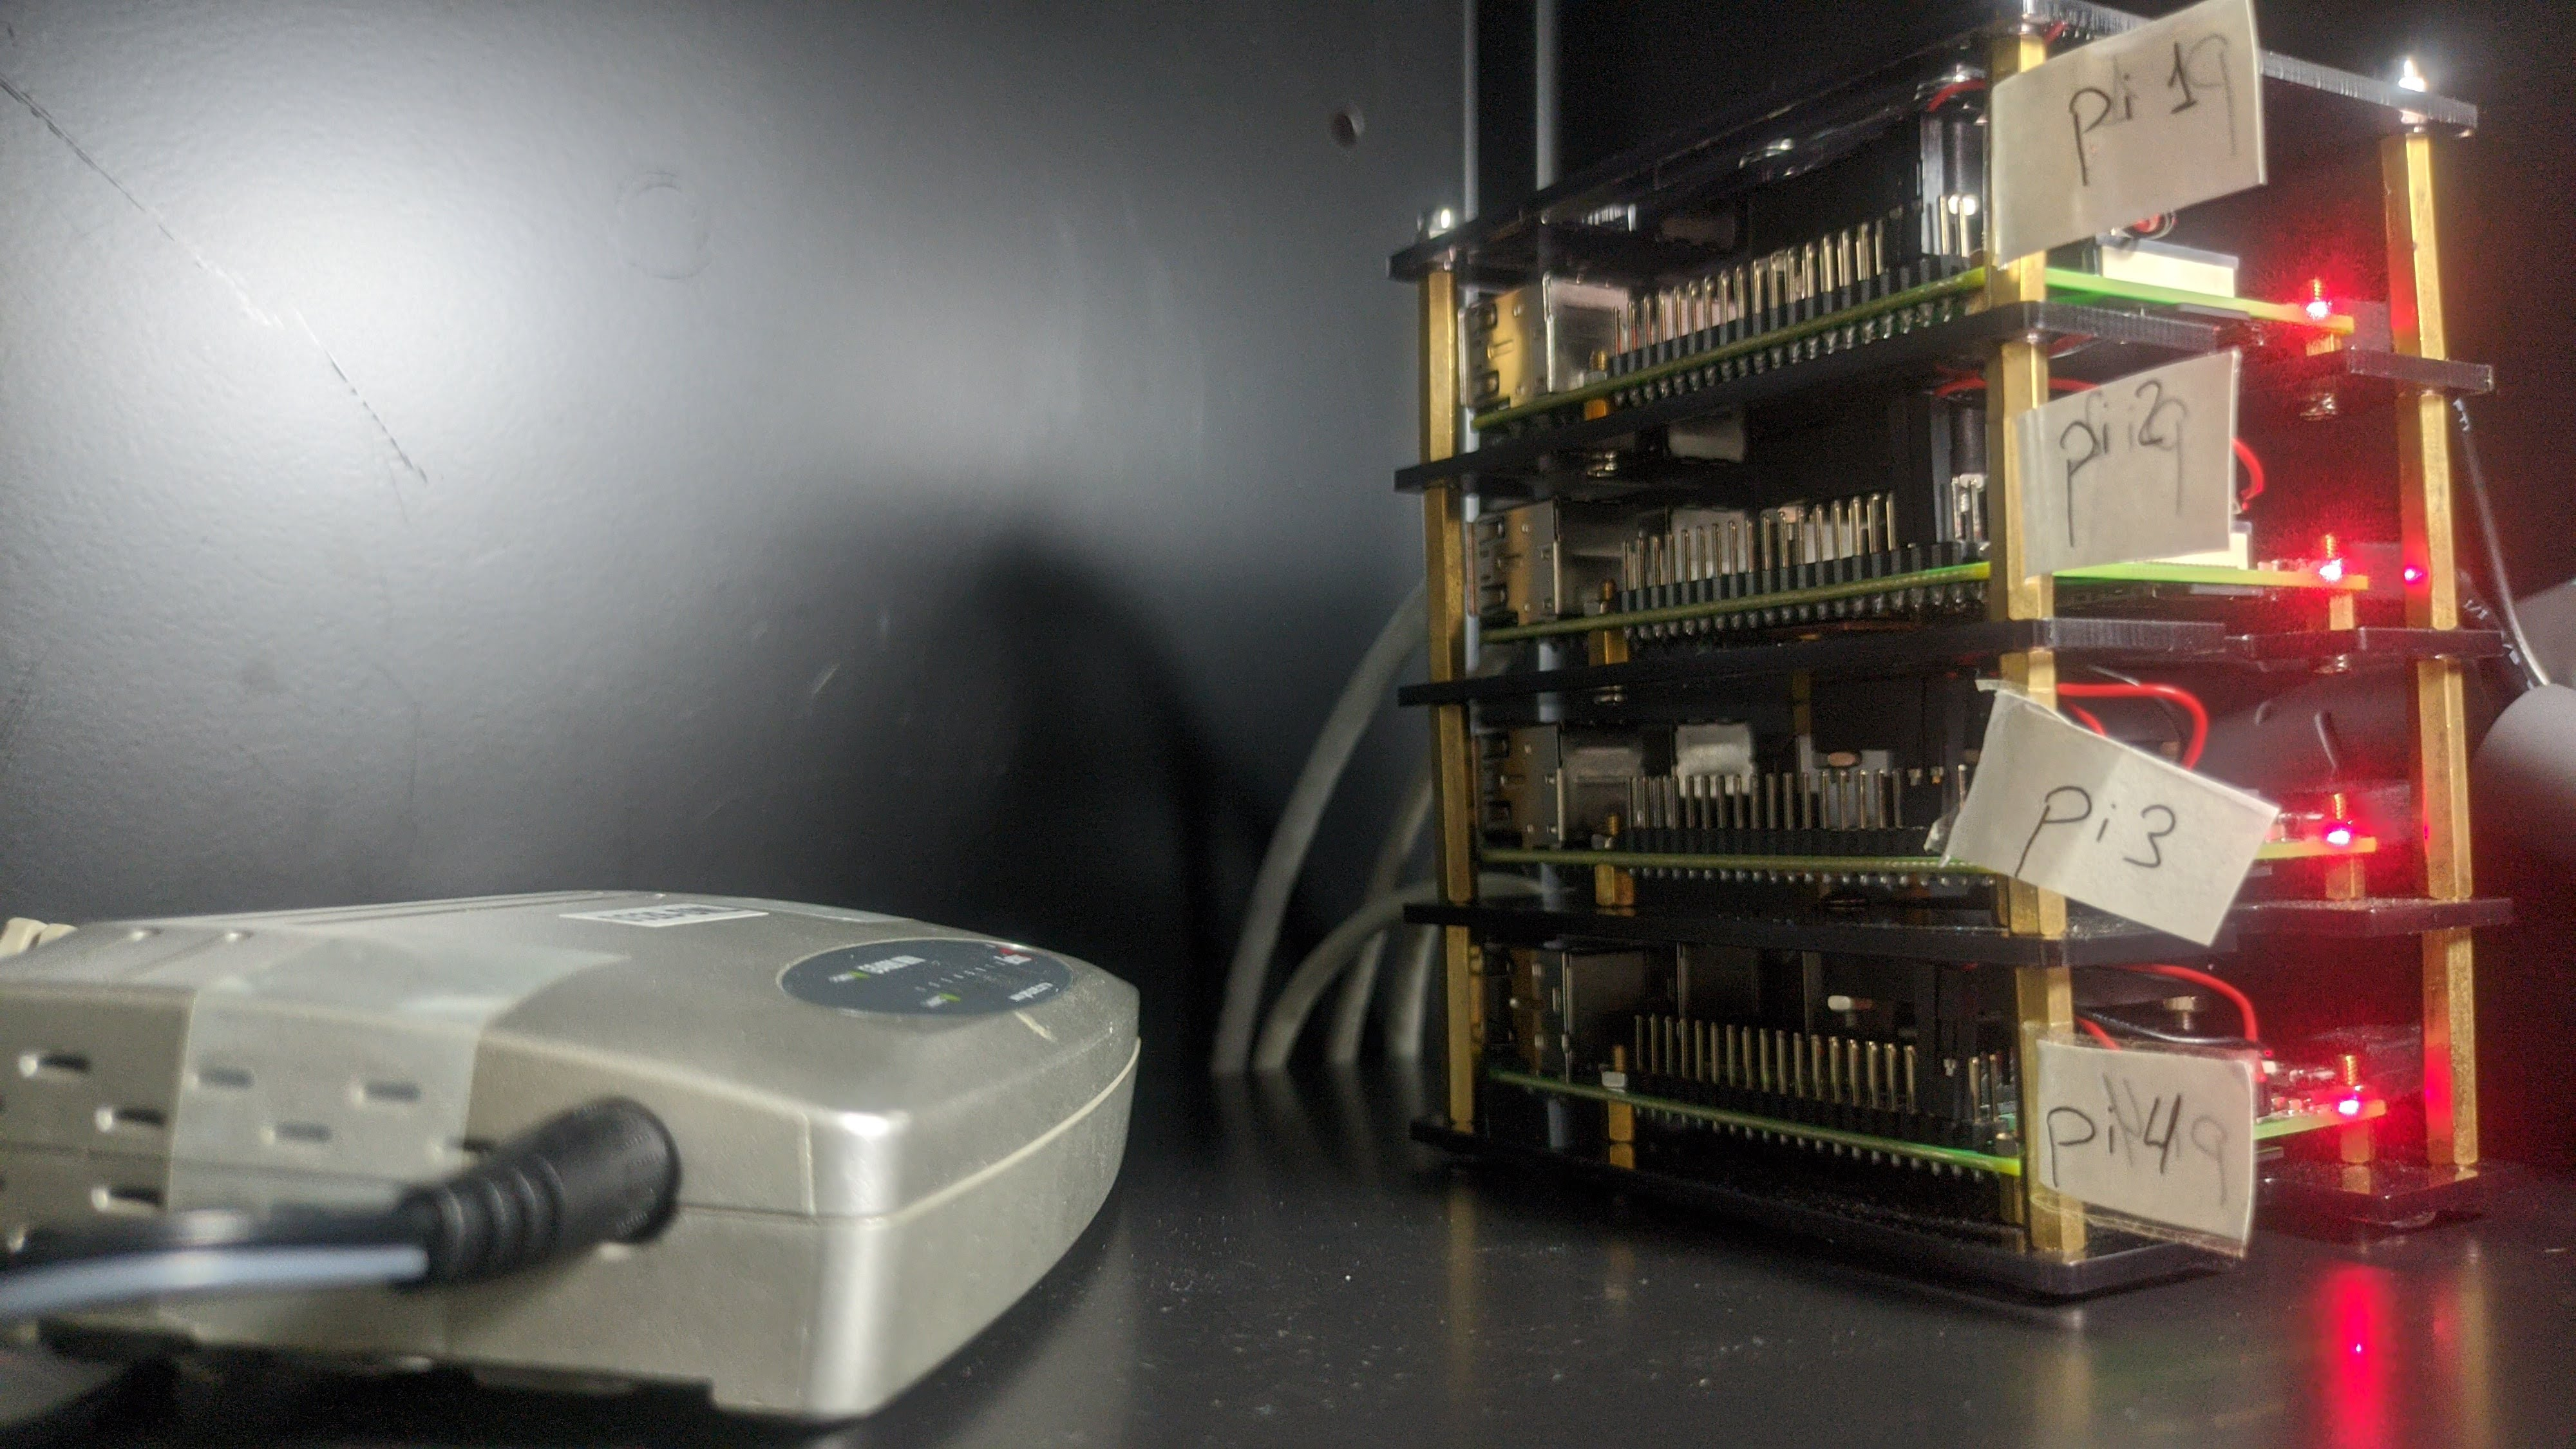
\includegraphics[width=0.75\textwidth]{Figuras/raspberrys.jpg}
    \caption{Montaje de las raspberrys}     
\end{figure}

La Jetson Nano y cada Raspberry tienen un cable ethernet conectado al switch, el cual a su vz cuenta con otro cable ethernet por el cual se conecta al router (no presente en las fotos).


% \newpage

% \subsection{Datos involucrados}
Al tratarse este proyecto de una modificación del sistema de recomendación de R.Sánchez y col., se heredarán todos los datos. Cabe mencionar que R.Sánchez y col. utilizaron información proporcionada por el proyecto Green Soul\autocite{EcoawarePersuasiveNetworked} para crear su sistema de recomendación. El proyecto Green Soul trataba de persuadir a los usuarios para que aumentase su conciencia energética y cambiaran sus hábitos de consumo, para ello, se realizaron una serie de encuestas donde se les preguntaba a los usuarios por sus datos personales y se les pedía que ordenarán en función de su criterio qué estrategias de persuasión les parecían más efectivas.
\\ \\
Por tanto, las estrategias de persuasión que se recomiendan pertenecen al ámbito de la concienciación del consumo energético, aunque podrían ser extrapolables a otros casos. De todas formas, se eludirán los detalles sobre estas estrategias ya que no son el caso de estudio y no entran en el alcance de este proyecto.
\\ \\
Teniendo en cuenta todo lo anterior, este capítulo se ha redactado para entender la gestión de los datos en este proyecto, ya que algunos son de carácter personal y es de suma importancia preservar su privacidad. Estos datos se pueden dividir en tres categorías:
\begin{itemize}
    \item \textbf{No sensibles}, la información de los elementos a recomendar, que no son ni personales ni suministrados por ninguna persona.
    \item  \textbf{Sensibles}, datos que hacen referencia a información personal o que son proporcionados por las personas involucradas en el cuestionario.
    \item \textbf{Sintéticos}, datos de usuarios generados aleatoriamente para paliar la necesidad de datos personales del modelo de consenso (sección \ref{Consenso}.Agregación de modelos por consenso).
\end{itemize} 

\subsubsection{No sensibles}
Como se ha mencionado antes, en la categoría de datos no sensibles se encuentran los datos que no son personales ni hacen referencia a ningún usuario. En esta categoría únicamente aparecen aquellos datos que hacen referencia a los elementos que se van a recomendar en el sistema y sus atributos.
\\ \\
Cada estrategia de persuasión que pueda recomendar el RS contará con hasta dos atributos, para que de esta forma, el sistema pueda conocer mejor las estrategias y realizar recomendaciones más precisas en base a esta información. En la tabla \ref{tab:EstrategiasPersuasion} se muestran las estrategias de persuasión involucradas en el RS y sus atributos.
\begin{table}[H]
    %Con esta función se inicia el entorno tabla, que se puede posicionar con respecto al texto al igual que una imagen.
    
    \begin{center}
    %Se centra la tabla.
        \begin{tabular}{|c|p{0.45\linewidth}|p{0.2\linewidth}|p{0.2\linewidth}|}
            % -------------
            \hline
            \rowcolor{Cyan} 
            % -------------
            \textbf{ID} & \textbf{Descripción} & \textbf{Atributo 1} & \textbf{Atributo 2} \\ 
            % -------------
            \hline
            \textbf{V2} &  Reconocimiento público/social de mi contribución al ahorro de energía. & Reconocimiento social & -\\
            % -------------
            \hline
            \rowcolor{GrisTabla}
            \textbf{V5} & Recibir información relacionada con la energía de una forma simple y estéticamente atractiva. & Atractivo físico & -\\
            % -------------
            \hline
            \textbf{V6} &  Recibir beneficios como recompensa por mejorar mi rendimiento energético(horarios de trabajo flexibles, saltarse ciertas tareas, etc.). & Condicionamiento & -\\
            % -------------
            \hline
            \rowcolor{GrisTabla} 
            \textbf{V7} & Recibir un reconocimiento por lograr ahorros de energía de manera colectiva yo y mi equipo. & Reciprocidad & Reconocimiento social\\
            % -------------
            \hline
            \textbf{V10} & Mis altos gerentes están comprometidos con el ahorro de energía. & Autoridad & Demostración social \\
            % -------------
            \hline
            \rowcolor{GrisTabla} 
            \textbf{V11} & Poder monitorear mi propio desempeño energético en tiempo real. & Monitorización propia. & - \\ 
            % -------------
            \hline
            \textbf{V15} &  Información sobre el efecto que mis acciones pueden tener sobre el consumo de energía. & Causa efecto & -\\
            % -------------
            \hline
            \rowcolor{GrisTabla} 
            \textbf{V17} & Evacuación comparativa de mi desempeño en el ahorro de energía respecto a usuarios parecidos a mí. & - & -\\
            % -------------
            \hline
            \textbf{V19} &  Consejos y sugerencias sobre el ahorro de energía al día o a la semana.  & Sugerencia & -\\
            % -------------
            \hline
            \rowcolor{GrisTabla} 
            \textbf{V20} &  Avances y consejos sobre las lecciones aprendidas de usuarios parecidos mí en acciones específicas de ahorro de energía. & Similaridad & -\\
            \hline

            % \rowcolor{Naranja} 
            % \textbf{V} & \textbf{elit} \\ \hline
        \end{tabular}
        \caption{\centering Estrategias de persuasión del sistema (Fuente: Elaboración propia).}
        \label{tab:EstrategiasPersuasion}
    \end{center}    
\end{table}


\subsubsection{Sensibles}
En cuanto a los datos sensibles hay que mencionar dos grupos, los datos personales de los usuarios y los rankings de los usuarios. Este primer grupo está formado por los datos personales de los usuarios participantes, que intervienen en dos puntos clave: en el entrenamiento de los modelos de IA y a la hora de agregar estos modelos. El grupo de los datos de los rankings está formado por las preferencias de los anteriores usuarios a la hora de ordenar las estrategias de persuasión, es decir, el ranking de estrategias para cada usuario.
\\ \\
Tanto los datos personales de los usuarios como los datos de los rankings de estos son necesarios para entrenar un modelo de IA. Los atributos de los usuarios, al igual que los atributos de las estrategias de persuasión, sirven para relacionar los distintos usuarios entre sí y encontrar relación entre sus diferentes atributos con el orden que le han dado a las diferentes estrategias de persuasión, de esta forma, se pueden realizar recomendaciones en base al tipo de usuario.

\paragraph{Datos de usuarios\\}
Los datos personales de los usuarios que intervienen en este proyecto son los presentes en la tabla \ref{tab:AtributosUsuarios}. Estos datos han sido transformados a objetos json para su posterior utilización, formando una lista de objetos en los que cada uno representa los datos personales de un usuario.
\begin{table}[H]
    %Con esta función se inicia el entorno tabla, que se puede posicionar con respecto al texto al igual que una imagen.
    
    \begin{center}
    %Se centra la tabla.
        \begin{tabular}{|c|c|p{0.7\linewidth}|}
            % -------------
            \hline
            \rowcolor{Cyan} 
            % -------------
            \textbf{ID} & \textbf{Nombre} & \textbf{Descripción}\\ 
            % -------------
            \hline
            \textbf{0} &  Edad & Rango de edad\\
            % -------------
            \hline
            \rowcolor{GrisTabla}
            \textbf{1} & Género & Género\\
            % -------------
            \hline
            \textbf{2} & Educación & Nivel educativo\\
            % -------------
            \hline
            \rowcolor{GrisTabla} 
            \textbf{3} & País & País de residencia\\
            % -------------
            \hline
            \textbf{4} & Cultura de trabajo & Cultura de trabajo\\
            % -------------
            \hline
            \rowcolor{GrisTabla} 
            \textbf{5} & PST & Tipo de perfil de usuario en base a los propuestos por Dan Lockton\autocite{locktonModelsUserDesigners2012} : \textit{"Pinball, Shortcut, Thought-ful"}\\ 
            % -------------
            \hline
            \textbf{6} & Barreras  & Barreras ante el cambio\\
            % -------------
            \hline
            \rowcolor{GrisTabla} 
            \textbf{7} & Intenciones & Intenciones ante el cambio\\
            % -------------
            \hline
            \textbf{8} & Confianza  & Confianza ante el cambio\\
            % -------------
            \hline

            % \rowcolor{Naranja} 
            % \textbf{V} & \textbf{elit} \\ \hline
        \end{tabular}
        \caption{\centering Atributos de los usuarios que participan en el sistema (Fuente: Elaboración propia).}
        \label{tab:AtributosUsuarios}
    \end{center}    
\end{table}
\paragraph{Rankings\\}
Los usuarios, a parte de introducir sus datos personales anteriores, también introducen el orden de las estrategias de persuasión en base a la relevancia que consideran que tienen. Este ranking de estrategia es recogido y transformado a formato json formando una lista de objetos json en la que cada objeto representa los datos de la tabla \ref{tab:RankingUsuario}.
\begin{table}[H]
    \begin{center}
    %Se centra la tabla.
        \begin{tabular}{|c|p{0.7\linewidth}|}
            % -------------
            \hline
            \rowcolor{Cyan} 
            % -------------
            \textbf{Nombre} & \textbf{Descripción}\\ 
            % -------------
            \hline
            \textbf{User ID}  & Identificador único del usuario\\
            % -------------
            \hline
            \rowcolor{GrisTabla}
            \textbf{Item ID}  & Identificador único de la estrategia de persuasión\\
            % -------------
            \hline
            \textbf{Ranking} & Valor en el ranking de la estrategia de persuasión\\
            % -------------
            \hline
            % \rowcolor{Naranja} 
            % \textbf{V} & \textbf{elit} \\ \hline
        \end{tabular}
        \caption{\centering Elementos de la estructura de los datos del ranking  (Fuente: Elaboración propia).}
        \label{tab:RankingUsuario}
    \end{center}    
\end{table}


\subsubsection{Sintéticos}
En cuanto a los datos sintéticos, se debe tener en cuenta que los datos sensibles han sido directamente suministrados por los usuarios, por lo cual, es técnicamente imposible acceder a ellos desde el servidor de agregación, ya que sería una evidente violación de la privacidad de los usuarios. Esto genera un gran problema debido a que el propio modelo de consenso, explicado en la sección \ref{Consenso}, requiere de datos de usuarios para funcionar.
\\ \\
La forma de abordar el problema de la necesidad de datos es mediante la creación de usuarios sintéticos, como se explica en la subsección \ref{Consenso:Usuarios_Sinteticos}. Estos usuarios sintéticos tendrán los mismos atributos que los usuarios normales (tabla \ref{tab:AtributosUsuarios}), tendrán que clasificar las mismas estrategias de persuasión (tabla \ref{tab:EstrategiasPersuasion}) y el ranking se gestionará de la misma forma (tabla \ref{tab:RankingUsuario}).


% \newpage

% \subsection{Protocolo de Federated Learning}\label{Protocolo}
El protocolo de Federated Learning que se va a reproducir en este proyecto es una adaptación de lo que proponen K. Bonawitz y col. \autocite{bonawitzFederatedLearningScale2019a}. En este protocolo se definen tres fases importantes, la selección de participantes, la configuración del mecanismo de agregación y el envío reporte de cada participante.
\\\\
Para este caso se han introducido leves cambios en este protocolo que se irán explicando en las sucesivas partes del mismo.  

\subsubsection{Selección de participantes}
La selección de participantes al tratarse de un caso de estudio concreto no se limita ni se controla de ninguna forma, simplemente se ha implementado una red en la que participan cuatro dispositivos diferentes.

\subsubsection{Intercambio de claves}
El intercambio de claves es una de las novedades introducidas sobre el protocolo previamente mencionado, en este paso, el objetivo es que los diferentes dispositivos de la red compartan sus claves públicas para poder asegurar la privacidad de la red, imagen \ref{fig:PublicKeyShare}. 
\\ \\
La utilización de estas claves públicas y su función están definidas en el apartado de securización de las comunicaciones \ref{SegCom}.
\begin{figure}[H]
    \centering
    \includegraphics[width=0.5\textwidth]{Figuras/Network_public_key.png}    
    \caption{Intercambio de claves públicas entre los participantes} 
    \label{fig:PublicKeyShare}
\end{figure}

\subsubsection{Entrenamiento}
El entrenamiento es algo que en el protocolo se omite pero que es importante mencionar. Este proceso se lleva a cabo en el dispositivo del participante y conlleva dos tareas:
\begin{itemize}
    \item En primer lugar este participante crea su modelo de IA, lo entrena con los datos que él elija y lo almacena.
    \item En segundo lugar este modelo es cifrado y enviado al servidor. El proceso de cifrado se puede observar en el diagrama \ref{fig:Flow_Encryption} de la sección de securización de las comunicaciones \ref{SegCom}.
\end{itemize} 
\begin{figure}[H]
    \centering
    \includegraphics[height=0.6\textheight]{Figuras/flowchart_train.png}    
    \caption{Intercambio de claves públicas entre los participantes} 
    \label{fig:Entrenamiento}
\end{figure}

\subsubsection{Comunicación con el servidor}
La comunicación con el servidor es un proceso crucial en el que se debe asegurar que los modelos de los participantes lleguen sin modificaciones y sin ser interceptados por ningún atacante. Para detallar este proceso se ha elaborado una sección donde se explican más a fondo los pasos llevados para conseguir que las comunicaciones sean seguras, sección \ref{SegCom}.
\\ \\
Debido a este protocolo de seguridad, los participantes deberán enviar tanto los modelos cifrados como las claves cifradas, acorde las siguientes imágenes.

\begin{figure}[H]
    \begin{minipage}[t]{0.45\linewidth}  % <---
        \centering
        \includegraphics[width=\textwidth]{Figuras/Network_participant_encrypted_key.png}
        \caption{Envío de la clave de cifrado del modelo al servidor de agregación} 
    \end{minipage}
    \hfill
    \begin{minipage}[t]{0.45\linewidth}  % <---
        \centering
        \includegraphics[width=\textwidth]{Figuras/Network_participant_encrypted_model.png}    
        \caption{Envío del modelo cifrado al servidor de agregación} 
    \end{minipage}
\end{figure}

\subsubsection{Agregación de los modelos}
En este proceso, como tal, no va a ocurrir una agregación de modelos, sino más bien una compartición de conocimiento de forma indirecta mediante el modelo de consenso. Este sistema está explicado con detalle en la sección \ref{Consenso} de este capítulo.
\\ \\
De todas formas, para verlo de una forma más sencilla, se puede observar el siguiente diagrama \ref{fig:Flow_Agregation} en el cual se muestra el flujo de los datos y de los modelos para ser agregados. El proceso que recorre este diagrama puede ser dividido en 4 partes:
\begin{itemize}
    \item Se reciben los modelos de los participantes (en este caso 4), se descifran siguiendo el diagrama \ref{fig:Flow_Decryption} (explicado con detalle en en la sección de securización de las comunicaciones \ref{SegCom}) y se guardan los modelos para su posterior utilización.
    \item Una vez se cuente con los modelos descifrados, se generan los usuarios sintéticos. Después, con el modelo de cada participante se realiza la predicción del ranking para estos usuarios y se almacena para su posterior utilización. 
    \item Mediante el modelo de consenso explicado en el apartado \ref{Consenso} estas predicciones son convertidas a una única predicción por usuario sintético generado. Después, la información se almacena para su uso final.
    \item Por último, se coge toda la información de los usuarios sintéticos y los rankings consensuados para reentrenar el modelo de cada participante. 
\end{itemize}
\begin{figure}[H]
    \centering
    \includegraphics[width=\textwidth]{Figuras/flowchart_agregation.png}    
    \caption{Diagrama del flujo de reentrenado de los modelos} 
    \label{fig:Flow_Agregation}
\end{figure}
\newpage
\subsubsection{Comunicación con los participantes}
La comunicación del servidor con los participantes se realiza de la misma forma en la que los participantes se comunican con el servidor. La única diferencia es que el receptor en este caso son los participantes y el emisor el servidor.
\begin{figure}[H]
    \begin{minipage}[t]{0.45\linewidth}  % <---
        \centering
        \includegraphics[width=\textwidth]{Figuras/Network_node_encrypted_key.png}
        \caption{Envío de la clave de cifrado del modelo de cada participante a cada participante} 
    \end{minipage}
    \hfill
    \begin{minipage}[t]{0.45\linewidth}  % <---
        \centering
        \includegraphics[width=\textwidth]{Figuras/Network_node_encrypted_model.png}    
        \caption{Envío de cada modelo cifrado a su correspondiente dueño} 
    \end{minipage}
\end{figure}
\subsubsection{Comparación de modelos}
En el momento que el modelo llega al participante, este tiene que valorar si realmente le supone una mejora o no. Para ello como puede verse en el diagrama \ref{fig:Flow_Compare}, existen varias fases a llevar a cabo.

En primer lugar, al igual que como con el servidor de agregación, se debe descifrar el modelo recibido. Después, compararlo con el modelo del participante. Esto se puede hacer tratando de analizar la precisión de las predicciones para varios subconjuntos de datos de test con los que cuente el dispositivo. En resumen, predecir para los usuarios existentes de su ranking con los dos modelos y quedarse con el modelo que más acierte.

\begin{figure}[H]
    \centering
    \includegraphics[height=0.6\textheight]{Figuras/flowchart_compare.png}    
    \caption{Diagrama del flujo de la comparación de los modelos} 
    \label{fig:Flow_Compare}
\end{figure}


% \newpage

% \subsection{Securización de las comunicaciones} \label{SegCom}
Para preservar la seguridad y privacidad durante las comunicaciones del protocolo de FL propuesto es imprescindible securizar las comunicaciones. Para securizar las comunicaciones se han llevado a cabo dos acciones clave, la primera en lo que concierne al protocolo de comunicación y la segunda en cuanto al cifrado de la comunicación.

\subsubsection{Protocolo de comunicación}
En cuanto al protocolo de comunicación, se ha optado por la utilización del protocolo SCP (Secure Copy Protocol), conocido en español como protocolo de copia segura. Este protocolo requiere del protocolo SSH (Secure Shell), conocido en español como terminal seguro.
\\ \\
El protocolo SSH permite el acceso remoto a un servidor o dispositivo por un canal seguro a través de una clave. Además, el protocolo usa técnicas de cifrado que impiden que la información que viaje en la red lo haga de forma legible. El protocolo SCP permite la transferencia de archivos entre dispositivos de la red usando el protocolo SSH como base.

\subsubsection{Cifrado de la comunicación}
Aunque las comunicaciones en el protocolo SCP y SSH vayan cifradas son susceptibles de ser atacadas. Para mejorar este aspecto se ha realizado un sistema de cifrado de los modelos que viajen por la red para preservar la privacidad y seguridad de los participantes.
\\ \\ 
Para esta labor se han utilizado el método criptográfico de criptografía híbrida, que usa tanto la criptografía simétrica como asimétrica.

\paragraph{Cifrado simétrico} 
El cifrado simétrico es aquel sistema de cifrado en el que la misma clave sirve para cifrar como para descifrar el mensaje. 
\\ \\
El problema de este sistema es que toda la seguridad reside en la clave empleada en el cifrado. Esto es un gran impedimento a la hora de gestionar comunicaciones debido al la forma de envíar la clave, ya que, si no se hace por un canal seguro, el mensaje sera fácilmente descifrable.
\\ \\
Por otro lado, este sistema cuenta con dos grandes ventajas, es sencillo, es rápido y requiere menos recursos para llevarlo a cabo.

\paragraph{Cifrado asimétrico}
El cifrado asimétrico es aquel sistema de cifrado que consta de dos claves criptográficas, una pública y una privada. La clave pública es utilizada para cifrar el mensaje, mientras que la privada es utilizada para descifrarlo. 
\\ \\
Este sistema cuenta con tres grandes desventajas que impiden su uso en exclusivo o su uso con grandes volúmenes de información a cifrar. 
\begin{itemize}
    \item Se necesita más procesado de cómputo para generar la clave.
    \item Las claves asimétricas son mucho más grandes que las simétricas.
    \item El mensaje cifrado ocupa más espacio que el original.
\end{itemize}

Debido a que los dispositivos con los que se cuenta no tienen una gran capacidad de cómputo no se podría establecer un tamaño de clave lo suficientemente grande como para poder cifrar el modelo de IA completo. Este modelo, pesa alrededor de los 7Kb y para cifrarlo con este sistema habría que generar una clave del mismo tamaño o mayor.
\\ \\
Sin embargo, este sistema al constar de dos claves independientes es más sencillo de implementar, puesto que no se envía la clave con la que se descifra el mensaje, sino con la que se cifra, lo que facilita la tarea y evita la búsqueda de canales seguros para enviar las cláves.

\paragraph{Cifrado híbrido}
Teniendo en cuenta los anteriores dos tipos de cifrado se decidió utilizar el sistema híbrido para obtener los resultados más óptimos, protegiendo la privacidad y pudiendo realizar las tareas de cifrado desde dispositivos con menor capacidad computacional.
\\ \\ 
El proceso de cifrado se ha realizado de acuerdo al diagrama de flujo representado en la figura \ref{fig:Flow_Encryption}. En este diagrama se pueden observar los pasos que se han realizado para la encriptación de la información, en primer lugar el modelo de LightFM se convirtió a bytes y se comprimió para reducir el volumen de datos a enviar por la red, pudiendo agilizar así las comunicaciones. Después se cifró simétricamente, generando una clave y un mensaje cifrado. Por un lado este mensaje cifrado sería comprimido y se guardaría en un fichero para su posterior envío. Mientras que por el otro lado, la clave de cifrado simétrica se encriptó asimétricamente con la clave pública del receptor del mensaje, dando como resultado una clave de cifrado simétrico cifrada asimétricamente. Esta clave sería guardada en un fichero para ser enviada al igual que el mensaje.
\begin{figure}[H]
    \centering
    \includegraphics[height=0.6\textheight]{Figuras/flowchart_encryption.png}    
    \caption{Diagrama de flujo del proceso de cifrado} 
    \label{fig:Flow_Encryption}
\end{figure}


\subsubsection{Descifrado del mensaje}
El descifrado del mensaje es el proceso inverso al cifrado de la figura \ref{fig:Flow_Encryption}. Para ello, en un primer momento se reciben tanto el modelo cifrado simétricamente como la clave del modelo cifrada asimétricamente. En primer lugar, la clave que se ha recibido se descifra asimétricamente con la clave privada propia, ya que esta sólo es descifrable por el receptor. Una vez descifrada la clave, se descomprime el modelo y se descifra con esta. Por último, el resultado es descomprimido y convertido a objeto LightFM para su posterior utilización. 
\begin{figure}[H]
    \centering
    \includegraphics[height=0.6\textheight]{Figuras/flowchart_decryption.png}    
    \caption{Diagrama de flujo del proceso de descifrado} 
    \label{fig:Flow_Decryption}
\end{figure}

% \newpage


\subsection{Agregación de modelos}\label{Consenso}

\subsubsection{Generar usuarios sintéticos}\label{Consenso:Usuarios_Sinteticos}


\subsubsection{Predecir ranking de los usuarios}

\subsubsection{Consensuar predicciones}

\subsubsection{Generar rankings sintéticos}

\subsubsection{Exportación de datos}

\subsubsection{Reentrenado}
% \newpage
% \cleardoublepage
% \input{Capitulos/8.4.Tecnologias}
% \newpage
% \cleardoublepage
% \input{Capitulos/8.5.ConsideracionesImplementacion}


\fancyhead[LE]{}
\newpage
\thispagestyle{empty}
\cleardoublepage

\chapter{Presupuesto}
\thispagestyle{fancy}
\fancyhead[LE]{\thechapter.Presupuesto} 
El presupuesto de este proyecto cuenta con dos apartados, el presupuesto de los materiales y el de los recursos humanos. Adicionalmente se ha añadido un apartado para explicar los requisitos de la plataforma de desarrollo, que al no ser adquirida para este proyecto no entra dentro de los costes, pero es un elemento fundamental para el desarrollo de software en este proyecto. 

\section{Plataforma de desarrollo}
Aunque el proyecto conste únicamente del gasto en materiales y recursos humanos se ha utilizado un ordenador de escritorio para su desarrollo. Aunque el presupuesto de este ordenador no sea exclusivo para el proyecto ha sido necesario para su desarrollo y para agilizar los despliegues y las pruebas. Además, este ordenador ha sido utilizado para desarrollar el código y probarlo, actividad que también ha agilizado mucho el desarrollo del proyecto.
\\ \\
Es por esto que, aunque no entre en el presupuesto, merecía ser mencionado. El ordenador cuenta con los diferentes componentes, tabla \ref{tab:PlataformaDesarrollo}.

\begin{table}[H]
    \begin{center}
    %Se centra la tabla.
        \begin{tabular}{|c|}
            % -------------
            \hline
            \rowcolor{Cyan} 
            \textbf{Plataforma de desarrollo} \\ 
            % -------------
            \hline
            \rowcolor{GrisTabla}
            \textbf{Ordenador de torre} \\
            \hline
            GPU: Nvidia GTX 970 \\
            \hline
            CPU: Ryzen 5 3600 \\
            \hline
            RAM: 16 gb \\
            % -------------
            \hline
        \end{tabular}
        \caption{\centering Presupuesto de los materiales utilizados.}
        \label{tab:PlataformaDesarrollo}
    \end{center}    
\end{table}


\newpage
\section{Materiales}
En cuanto al presupuesto de los materiales que se han utilizado en el proyecto, se ha elaborado la tabla \ref{tab:PresupuestoMateriales} donde se detalla tanto la lista de materiales, como su precio.
\\ \\
Este presupuesto está agrupado en 5 categorías, las Raspberries Pi, las tarjetas SD, la Jetson Nano, los cables y los elementos de telecomunicación. Esta clasificación permite observar en qué grupos se ha gastado más. 

\begin{table}[H]
    \begin{center}
    %Se centra la tabla.
        \begin{tabular}{|r|c|r|r|}
            % -------------
            \hline
            \rowcolor{Cyan} 
            % -------------
            \multicolumn{4}{|c|}{\textbf{Materiales}}\\
            \hline
            \textbf{Hardware} & \textbf{Cantidad} & \textbf{Precio unidad}& \textbf{Precio total}\\ 
            % -------------
            \hline
            \rowcolor{GrisTabla}
            \textbf{Raspberries} &  \textbf{5} & & \textbf{185,40 \euro}\\
            Pi 3 B & 1 & 37,44 \euro & 37,44 \euro\\
            Pi 3 B+ & 4 & 36,99 \euro & 147,96 \euro\\
            % -------------
            \hline
            \rowcolor{GrisTabla}
            \textbf{SD-s} &  \textbf{8} & & \textbf{50 \euro}\\
            16 GB & 1 & 6 \euro & 42 \euro\\
            32 GB & 4 & 8 \euro & 8 \euro\\
            % -------------
            \hline
            \rowcolor{GrisTabla}
            \textbf{Jetson Nano} & \textbf{1} & & \textbf{140 \euro}\\
            NVIDIA Jetson Nano & 1 & 140 \euro & 140 \euro\\
            % -------------
            \hline
            \rowcolor{GrisTabla}
            \textbf{Cables} &  \textbf{5} & & \textbf{137 \euro}\\
            Alimentación Raspberry & 5 & 10 \euro & 50\euro\\
            Alimentación Jetson Nano & 1 & 15 \euro & 15 \euro\\
            Regleta enchufes & 2 & 10 \euro & 10 \euro\\
            Rack Raspberries & 1 & 20 \euro & 20 \euro\\
            RJ45 & 8 & 4 \euro & 32 \euro\\
            % -------------
            \hline
            \rowcolor{GrisTabla}
            \textbf{Telecomunicaciones} &  \textbf{2} & & \textbf{29,41} \euro\\
            Switch & 1 & 11 \euro & 11 \euro\\
            Router & 1 & 18,41 \euro & 18,41 \euro\\
            % -------------
            \hline
            \rowcolor{Naranja} 
            % -------------
            \multicolumn{3}{|r}{\textbf{Total}} & \textbf{541,81 \euro}\\
            \hline
            % \rowcolor{Naranja} 
            % \textbf{V} & \textbf{elit} \\ \hline
        \end{tabular}
        \caption{\centering Presupuesto de los materiales utilizados.}
        \label{tab:PresupuestoMateriales}
    \end{center}    
\end{table}


\newpage
\section{Recursos Humanos}
En cuanto a los recursos humanos que intervienen en el proyecto se ha decidido contar con los siguientes tipos de especialistas que, desempeñando estos roles, desarrollarán el proyecto.

\begin{table}[H]
    \begin{center}
    %Se centra la tabla.
        \begin{tabular}{|l|c|p{0.4\linewidth}|}
            % -------------
            \hline
            \rowcolor{Cyan} 
            \textbf{Perfiles} & \textbf{Precio hora} & \textbf{Responsabilidades} \\ 
            % -------------
            \hline
            \rowcolor{GrisTabla}
            & & $\bullet$ Organización\\
            \rowcolor{GrisTabla}
            & & $\bullet$ Gestión\\
            \rowcolor{GrisTabla}
            & & $\bullet$ Delimitar alcance y objetivos\\
            \rowcolor{GrisTabla}
            \multirow{-4}{*}{\textbf{Jefe de proyecto}} & \multirow{-4}{*}{\textbf{45 \euro}} & $\bullet$ Búsqueda de tecnologías\\
            \hline

            & & $\bullet$ Realización de la memoria técnica\\
            & & $\bullet$ Preparación de la defensa\\
            & & $\bullet$ Entre e impresión de la memoria y defensa\\
            \multirow{-4}{*}{\textbf{Analista de software interno}} & \multirow{-4}{*}{\textbf{30 \euro}} & $\bullet$ Búsqueda de nuevas tecnologías\\
            \hline

            \rowcolor{GrisTabla}
            & & $\bullet$ Ideas sobre cómo afrontar problemas\\
            \rowcolor{GrisTabla}
            & & $\bullet$ Resolver dudas\\
            \rowcolor{GrisTabla}
            & & $\bullet$ Presentar sistema de recomendación anterior\\
            \rowcolor{GrisTabla}
            \multirow{-4}{*}{\textbf{Analista de software externo}} & \multirow{-4}{*}{\textbf{30 \euro}} & $\bullet$ Consejos\\
            \hline

            & & $\bullet$ Idear la estructura del modelo de consenso\\
            & & $\bullet$ Desarrollar el protocolo de federated learning\\
            \multirow{-3}{*}{\textbf{Arquitecto de software}} & \multirow{-3}{*}{\textbf{45 \euro}} & $\bullet$ Planificar conexiones entre dispositivos y requisito\\
            \hline

                
            % -------------
            \rowcolor{GrisTabla}
            \textbf{Desarrollador de software} & \textbf{35 \euro} & $\bullet$  Programación del proyecto\\
            \hline

            & & $\bullet$ Revisar gramática de la memoria\\
            & & $\bullet$ Revisar el software desarrollado\\
            \multirow{-3}{*}{\textbf{Gestor de calidad}} & \multirow{-3}{*}{\textbf{30 \euro}} & $\bullet$ Revisión de bugs y errores\\
            \hline

        \end{tabular}
        \caption{\centering Precio hora de los distintos perfiles que intervienen en el proyecto.}
        \label{tab:PrecioPerfil}
    \end{center}    
\end{table}
\pagebreak
Estos roles de la tabla \ref{tab:PrecioPerfil} serán interpretados por los siguientes colaboradores del proyecto, presentes en la tabla \ref{tab:PersonaPerfil}. Cabe destacar que el rol de analista interno solo será llevado a cabo por Ibai Guillén, el resto de participantes, en caso de desempeñarlo, ejercerán de analistas externos.
\begin{table}[H]
    \begin{center}
        %Se centra la tabla.
        \begin{adjustbox}{angle=90}  
                \begin{tabular}{|p{0.22\linewidth}|p{0.12\linewidth}|p{0.12\linewidth}|p{0.15\linewidth}|p{0.19\linewidth}|p{0.135\linewidth}|}
                    % -------------
                    \hline
                    \rowcolor{Cyan} 
                    \backslashbox{Personas}{Perfiles} & \textbf{Jefe de proyecto} & \textbf{Analista} & \textbf{Arquitecto} & \textbf{Desarrollador} & \textbf{Gestor de calidad}\\ 
                    % -------------
                    \hline
                    \rowcolor{GrisTabla}
                    \textbf{Oihane Gómez} &  & 2 horas &  &  & \\
                    % -------------
                    \hline
                    \textbf{Rubén Sánchez} &  & 3 horas &  &  & \\
                    % -------------
                    \hline
                    \rowcolor{GrisTabla}
                    \textbf{Diego Casado} & 6 horas & 8 horas & 6 horas &  & 4 horas\\
                    % -------------
                    \hline
                    \textbf{Ibai Guillén} & 40 horas & 100 horas & 50 horas & 110 horas & 32 horas\\
                    \hline
                \end{tabular}
        \end{adjustbox}  
        \caption{\centering Horas de cada persona en cada labor} \label{tab:PersonaPerfil}
  
    \end{center}
\end{table}%

El presupuesto para esta plantilla sería el producto de las horas que han dedicado las personas de la tabla \ref{tab:PersonaPerfil} con el precio hora de la tabla \ref{tab:PrecioPerfil}. Esto queda reflejado en la siguiente tabla \ref{tab:PresupuestoRRHH}.

\begin{table}[H]
    \begin{center}
    %Se centra la tabla.
        \begin{tabular}{|c|c|}
            % -------------
            \hline
            \rowcolor{Cyan} 
            \textbf{Persona} & \textbf{Coste total} \\ 
            % -------------
            \hline
            \rowcolor{GrisTabla}
            Oihane Gómez & 60 \euro\\
            \hline
            Rubén Sánchez & 90 \euro\\
            \hline
            \rowcolor{GrisTabla}
            Diego Casado & 900 \euro\\
            \hline
            Ibai Guillén & 15.010 \euro\\
            \hline
            \rowcolor{Naranja}
            \textbf{Total} & \textbf{16.060 \euro}\\
            \hline
            % -------------
        \end{tabular}
        \caption{\centering Presupuesto total de RRHH.}
        \label{tab:PresupuestoRRHH}
    \end{center}    
\end{table}

\fancyhead[LE]{}
\newpage
\thispagestyle{empty}
\cleardoublepage

\chapter{Conclusiones y trabajo futuro}
\thispagestyle{fancy}
\fancyhead[LE]{\thechapter.Conclusiones y trabajo futuro}

En cuanto a las conclusiones queda claro que el FL es una tecnología habilitadora que permite distribuir el ML. Hay que tener en cuenta que la separación de los datos en ocasiones puede traer mejoras de rendimiento asociadas.
\\\\
En los sistemas de FL la agregación se realiza pidiendo a cada participante que envíe unos hiperparámetros de su modelo para poder usarlos para crear el modelo global, el objetivo que se persigue en este proyecto es un cambio de enfoque en la agregación y afrontarla desde el reentrenado de los modelos de cada participante. El reentrenado permite que cada participante se beneficie individualmente sin compartir ningún elemento de su modelo, funcionamiento que viene bien para evitar ataques de envenenamiento de datos o modelo, ya que es difícil que infiera en los demás participantes.
\\\\
Además, el reentrenado evita que un participante cuando reciba el modelo trate de averiguar información sobre otros modelos ya que no dispone de esta información. 
\\\\
Otro punto a considerar es que el FL agregado por modelo de consenso permite que no haya que desarrollar todos los modelos sobre el mismo framework, al contrario que con los sistemas existentes el consenso no necesita de métodos propios de un tipo concreto de objeto, lo que permite que haya redes con modelos heterogéneos de distintas librerías que puedan participar y beneficiarse de la misma forma.
\\\\
Lo más positivo de este sistema es que cada participante tiene su propio modelo y su propia información y solo él decide con qué información entrenar el modelo que quiere compartir. De esta forma cada participante es libre de definir la información sensible que no quiere utilizar o la información de usuarios que han expresado su negativa expresa. 
\\\\
En cuanto a la agregación todavía existen posibilidades no exploradas a la hora de realizar una función de consenso más eficaz, en este proyecto se ha partido de la moda y mediana estadísticas para la realización del estudio sobre el sistema, pero en lo que se refiere a la función se podrían desarrollar otras soluciones que tuvieran más elementos en cuenta para aumentar su precisión.
\\\\
Las comunicaciones ya eran un reto del FL y en este proyecto aunque se ha tratado de solventarlo ligeramente con compresión y encriptado el flujo de red es bastante grande. Con el objetivo de reducir el tamaño de las comunicaciones se podrían estudiar distintos algoritmos de compresión o minimizar el tamaño del modelo.

\fancyhead[LE]{}
\newpage
\thispagestyle{empty}
\cleardoublepage

\printbibliography

\appendix

\appendix

%\appendixname %nombre del capitulo como índice
\chapter{Protección de Datos en la Unión Europea y España}\label{appendix:ProteccionDatos}
\thispagestyle{fancy}
\fancyhead[LE]{Apéndice \thechapter.Protección de Datos en la Unión Europea y España} 
\begin{refsection}

\section{Preludio}
Ante la llegada de las Tecnologías de la Información y la Comunicación (TIC), la Organización para la Cooperación y el Desarrollo Económicos (OCDE) decidió definir unas directrices el 23 de septiembre de 1980 que regulen \textit{".. la protección de la privacidad y el flujo transfronterizo de datos personales ... "} \autocite[\ppno 1]{oecdOECDGuidelinesProtection2002}. Este fue uno de los primeros intentos de regular la gestión y utilización de los datos personales.
\\ \\
No llegaron medidas concretas a Europa hasta el 24 de octubre de 1995, cuando el Parlamento Europeo y el Consejo Europeo publicaron la \textit{"Directiva 95/46/CE"} \autocite{DIRECTIVA9546} con el objetivo de crear un marco jurídico que garantizase la protección de los datos y la libre circulación de estos. Por eso, en España se creó la \textit{"Ley Orgánica 15/1999, de 13 de diciembre, de Protección de Datos de Carácter Personal"} \autocite{LEYORGANICA15} más conocida por sus siglas LOPD, que era la encargada de garantizar el cumplimiento de la directiva europea en España. 
\\ \\
Ante la ausencia de leyes que garantizaran el cumplimiento de los derechos humanos en internet, algunos autores empezaron a definir los derechos digitales. Una de las primeras declaraciones de derechos fundamentales tecnológicos fue la de Robert B. Gelman, que en 1997 difundió una propuesta de \textit{"Declaración de los Derechos Humanos en el Ciberespacio"}, basada en la Declaración Universal de los Derechos Humanos de 1948.
\\ \\
Sin embargo, aunque el trabajo de Robert B. Gelman fue ampliamente apoyado por una gran comunidad de expertos, no ha sido hasta la entrada en el siglo XXI (cuando las TIC ya han conseguido una gran relevancia en la sociedad) que se ha empezado a atisbar la necesidad de derechos digitales inherentes de vivir en una sociedad tecnológica. Tanto es así, que varios autores empezaron a escribir sobre la necesidad de una nueva generación de derechos humanos que incluyese el campo de la tecnología.
\\ \\
La corriente pro derechos digitales llegó inclusive a la Unión Europea, que en el año 2000 redactó la \textit{"Carta de los Derechos Fundamentales de la Unión Europea"} \autocite{CartaDerechosFundamentalesb} en Niza con el objetivo de \textit{"... reforzar la protección de los derechos fundamentales a tenor de la evolución de la sociedad, del progreso social y de los avances científicos y tecnológicos."} \autocite[\ppno 5]{CartaDerechosFundamentalesb}. El problema es que no pasó a ser jurídicamente vinculante hasta el año 2009 junto con el Tratado de Lisboa. Esta carta es especialmente innovadora en cuanto a la protección de datos de carácter personal, puesto que establecía como derecho fundamental la protección de estos en el artículo 8. En este artículo se establecía que además, estos se tratarían de modo leal y con el consentimiento de la persona afectada. Asimismo, la persona afectada tendría derecho a acceder a los datos recogidos, así como a la rectificación de los mismos.

\section{Legislación}\label{appendix:ProteccionDatos_Legislacion}
La legislación vigente en Europa cambió radicalmente en el 2016, el parlamento europeo adoptó nuevas medidas para la era digital.
\\ \\
El 5 de mayo de 2016 entró en vigor la Directiva (UE) 2016/680 \autocite{DIRECTIVAUE2016}, reconocida como la Directiva sobre protección de datos en el ámbito penal, \textit{"... relativa a la protección de las personas físicas en lo que respecta al tratamiento de datos personales por parte de las autoridades competentes para fines de prevención, investigación, detección o enjuiciamiento de infracciones penales o de ejecución de sanciones penales, y a la libre circulación de dichos datos ..."} \autocite[\ppno 1]{DIRECTIVAUE2016}. La Comisión Europea define esta medida en su página web \autocite{ProteccionDatosUEa} como:

\begin{minipage}[t]{0.2\linewidth}
\end{minipage}
\hfill
\begin{minipage}[t]{0.9\linewidth}
  \textit{"... protege el derecho fundamental de los ciudadanos a la protección de sus datos cuando los utilicen las autoridades policiales y judiciales a efectos de aplicación de la ley. Más concretamente, la Directiva garantizará que se protejan adecuadamente los datos personales de víctimas, testigos y sospechosos de delitos, además de facilitar la cooperación transfronteriza en la lucha contra la delincuencia y el terrorismo."}
\end{minipage}
\\ \\ \\
El 24 de mayo de 2016 el Reglamento (UE) 2016/679 \autocite{REGLAMENTOUE2016}, reconocido como el Reglamento General de Protección de Datos (RGPD). \textit{"... relativo a la protección de las personas físicas en lo que respecta al tratamiento de datos personales y a la libre circulación de estos datos …"} \autocite[\ppno 2]{REGLAMENTOUE2016}. La Comisión Europea define esta medida en su página web como:

\begin{minipage}[t]{0.2\linewidth}
\end{minipage}
\hfill
\begin{minipage}[t]{0.9\linewidth}
  \textit{"... es una medida esencial para fortalecer los derechos fundamentales de las personas en la era digital y facilitar la actividad económica, ya que aclara las normas aplicables a las empresas y los organismos públicos en el mercado único digital. Además, la existencia de una norma única pone fin a la fragmentación en distintos sistemas nacionales y a las cargas administrativas innecesarias."}
\end{minipage}
\\ \\ \\
Esta legislación no sería aplicable hasta dos años más tarde, el 6 y 25 de mayo de 2018 respectivamente. Dos años durante los cuales cualquier empresa de la unión o cualquier empresa que tenga negocios en la Unión Europea se debía adaptar a la nueva normativa.
\\ \\
El objetivo principal de este reglamento era proteger a las personas físicas en cuanto al tratamiento de sus datos personales y a la libre circulación de estos. Estos datos son de naturaleza sensible, puesto que pueden revelar la identidad de la persona, ya sea mediante el nombre completo, la dirección de su domicilio, el número de tarjeta bancaria, etc.
\\ \\
Entre las cuestiones más relevantes del RGPD destacan: 
\begin{itemize}
  \item La transparencia: obliga a las organizaciones a comunicar a los usuarios el tratamiento que se realiza a sus datos.
  \item El derecho a la rectificación y borrado: cada usuario tendrá derecho a pedir que se rectifiquen sus datos en caso de ser inexactos. Además, los usuarios tendrán derecho a que las organizaciones borren sus datos y rescindir el consentimiento de tratamiento de ellos.
  \item Derechos sobre el procesamiento: cada usuario podrá solicitar la limitación de procesamiento de sus datos, así como negarse a que se usen en tomas de decisiones o en perfiles automatizados, aparte, también podrá solicitar que le entreguen sus datos en formato estructurado cuando sea posible.
\end{itemize}
La directiva sobre protección de datos en el ámbito penal y el RGPD dejaron obsoleta la LOPD española, por lo cual, para adaptarse al nuevo marco jurídico europeo el 7 de diciembre de 2018 entró en vigor la \textit{"Ley Orgánica 3/2018, de 5 de diciembre, de Protección de Datos Personales y Garantía de los Derechos Digitales"} \cite{samperLeyOrganica20182020} (LOPD-GDD), acorde con el RGPD.
\\ \\
Esta ley transpone el RGPD europeo a la legislación española, incluyendo medidas como:
\begin{itemize}
  \item La incorporación del término privacidad desde el diseño, lo que quiere decir que deben elaborarse procesos empresariales teniendo en cuenta la LOPD-GDD desde un primer momento. 
  \item El consentimiento, donde se obliga a las organizaciones a obtener el consentimiento explícito para el tratamiento de datos de las personas, estas personas, además, podrán solicitar la portabilidad de sus datos o la eliminación de los mismos.
  \item Sin embargo, la LOPD-GDD no se ciñe únicamente a adaptar el RGPD a la legislación Española, fue la primera ley europea de protección de datos en incluir explícitamente los derechos digitales de las personas en los entornos digitales.
\end{itemize}

\section{Derechos fundamentales}\label{appendix:ProteccionDatos_Derechos}

Como se ha comentado en el apartado anterior, con la entrada en vigor de la LOPD-GDD España se convirtió en el primer país europeo en garantizar los derechos digitales. Estos derechos digitales llegaron en 2018 en el Título X de la LOPD-GDD, titulado \textit{"Garantía de los derechos digitales"}, en respuesta a la Carta de los Derechos Fundamentales de la Unión Europea y a las nuevas medidas del Reglamento (UE) 2016/679 y de la Directiva (UE) 2016/680. 
\\ \\
Varios de los derechos recogidos en la LOPD-GDD fueron:
\begin{itemize}
  \item El derecho a la intimidad y uso de dispositivos digitales en el ámbito laboral.
  \item El derecho a la desconexión digital en el ámbito laboral.
  \item Derecho al olvido en búsquedas de Internet.
  \item El derecho al testamento digital.
\end{itemize}
Este paso adelante por parte del estado español incentivó a que un año después de la entrada en vigor de la LOPD-GDD, el Ilustre Colegio de la Abogacía de Barcelona (ICAB) presentase la \textit{"Carta de Barcelona por los Derechos de la Ciudadanía en la Era Digital"} \autocite{CartaBarcelonaPor}, apoyada por universidades y entidades de la sociedad civil. 
\\ \\
A la vista de la relevancia e impacto del tema, el gobierno español (representado por el Ministerio de Asuntos Económicos y Transformación Digital), se inspirará en la carta del ICAB para redactar la pionera \textit{"Carta de Derechos Digitales"} \autocite{CartaDerechosDigitales} de España, que contribuirá con los objetivos ya avanzados en el Título X de la LOPD-GDD. Se prevé que sea aprobada antes de 2022 para la estrategia España Digital 2025.
\\ \\
Esta carta cuenta con 25 puntos de alta relevancia entre los que están los recogidos en el anteriormente mencionado Título X de la LOPD-GDD, y entre otros, algunos de especial impacto en el desarrollo de este proyecto: los derechos ante la Inteligencia Artificial (Derecho XXIII) y el derecho a no ser localizado y perfilado (Derecho V). 
\\ \\
El derecho a no ser localizado y perfilado deja claro que cada persona tiene derecho a la \textit{"... libre autodeterminación individual (...) a no ser objeto de localización, ni a ser sometido a análisis de la personalidad o conducta que impliquen el perfilado de la persona"}, además, añade que sólo se podrán realizar \textit{"... tratamientos de información personal con el consentimiento de la persona afectada ..."}.
\\ \\
En cuanto al derecho ante la Inteligencia Artificial expone como primer punto que, en lo que concierne al desarrollo y ciclo de vida de esta, \textit{"Se deberá garantizar el derecho a la no discriminación algorítmica …"}. Además. en procesos de decisión automatizada las personas tienen derecho a \textit{"Solicitar una supervisión e intervención humana"} o \textit{"Impugnar las decisiones automatizadas o algorítmicas"}.
\\ \\
La carta, al no estar aprobada aún, no es legalmente vinculante, por lo que no es de obligado cumplimiento. Sin embargo, deja clara la orientación que van a tomar los derechos digitales en los próximos años.

\newpage
\thispagestyle{empty}
\cleardoublepage
\printbibliography[heading=subbibliography]

\end{refsection}

\fancyhead[LE]{}
\newpage
\thispagestyle{empty}
\cleardoublepage

%\appendixname %nombre del capitulo como índice
\chapter{Documentos adicionales}\label{appendix:Documentos}
\thispagestyle{fancy}
\fancyhead[LE]{Apéndice \thechapter.Documentos adicionales} 
En este apartado se adjuntan los documentos que debido a su tamaño puede que no se puedan observar con claridad en la memoria del proyecto.

\section{Planificación del Proyecto}\label{appendix:Documentos_Planificacion}
En la siguiente hoja se adjunta el diagrama GANTT de la planificación del proyecto a tamaño completo.
\newpage
\thispagestyle{empty}
\includepdf[angle=90]{PDF/GanttPlanificacion}

\fancyhead[LE]{}
\newpage
\thispagestyle{empty}
\cleardoublepage


\end{document}
%Función de final de documento.

%Acuda a continuación a leer los comentarios de los capítulos de introducción, objetivos y sobretodo aquellos del archivo de funciones.


%%%%%%%%%%%%%%%%%%%%%%%%%%%%%%%%%%%%%%%%%%%%%%%%%%%%%%%
%%%%%%%%%%%%%%%%%%%%%%%% FINAL %%%%%%%%%%%%%%%%%%%%%%%%
%%%%%%%%%%%%%%%%%%%%%%%%%%%%%%%%%%%%%%%%%%%%%%%%%%%%%%%

%Sin nada más que añadir, espero que les haya sido de gran utilidad esta plantilla y que gracias a ellan puedan adentrarse en el mundo del LATEX.

%Un saludo y mucho ánimo con la redacción y con el grado, falta muy poco.

%Miguel González Moreno